\chapter{Aktueller Stand}

In diesem Kapitel wird der \cob vorgestellt und auf die Unterschiede der
einzelnen Distributionen sowie zu anderen von \ac{IPA} eingegangen. Desweiteren
wird ein Überblick über \ac{ROS} als Framework für Roboter gegeben. Zuletzt
werden der bisherige Kalibrierablauf und dessen Schwächen dargestellt.

\section{Aufbau und Beschreibung des \cob}

Das Projekt \cob wurde vom \ac{IPA} bereits 1998 ins Leben gerufen. Bisher sind
daraus drei Robotergenerationen hervorgegangen. Von der aktuellen dritten
Generation gibt es bislang 7 Modelle, von denen zwei in Stuttgart am \ac{IPA}
eingesetzt werden. Dies sind die beiden Modelle cob3-3 und cob3-6. Die anderen
Modelle wurden an externe Forschungseinrichtungen verkauft und waren für Tests
an der Hardware nicht verfügbar. Der Grundaufbau ist für jeden \cob der dritten
Generation der selbe und in  am Beispiel des \cob 3-2 in Abbildung \ref{setup} dargestellt.

\begin{figure}[ht]
\centering
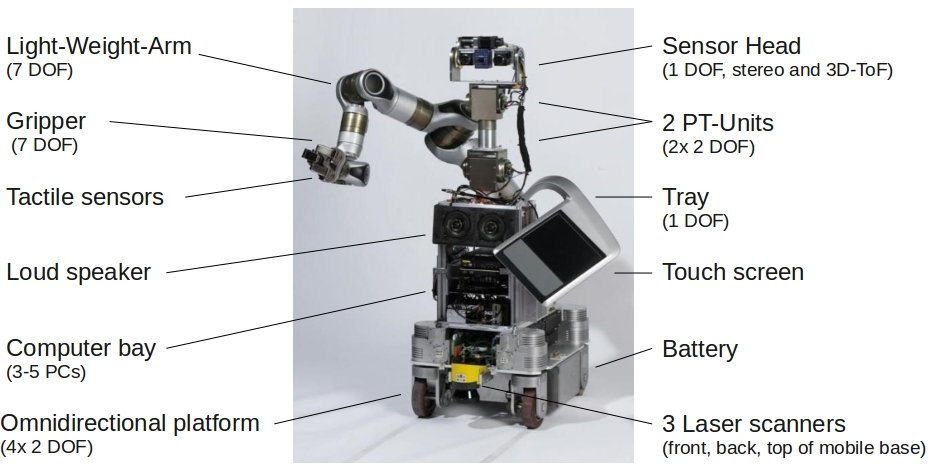
\includegraphics[width=\textwidth]{images/hw_setup_with_text}
\caption{Hardwarekomponenten des \cob}
\label{setup}
\end{figure}

  Die einzelnen Modelle unterscheiden sich aber in ihren
eingesetzten Komponenten. So ist der offensichtlichste Unterschied zwischen
den in /missingfigure{cob3-3 und cob3-6} abgebildeten cob3-3 und cob3-6 der von verschiedenen Herstellern stammende Arm. 

\subsection{Aktoren}

Die an den verschiedenen \cob Distributionen sind mit den folgenden Aktoren
ausgestattet, zu denen auch die Unterschiede der Modellnummern cob3-3 und
cob3-6 aufgelistet sind.

\begin{description}
  \item[Arm] Für den an der Rückseite des Roboters
    angebrachten Arm werden zwei Modelle eingesetzt. Einmal der \ac{LBR3} von
    Kuka sowie der \ac{LWA} von Schunk. 
  \item[Torso] Der Torso ist je nach
    Modellnummer ein 3 \ac{DOF} oder ein 4 \ac{DOF} Modell. Sowohl beim \cob
    3-3 als auch beim \cob 3-6 wird das 3 \ac{DOF} Modell eingesetzt.
  \item[Base] Als Basis für den Roboter dient eine Omnidirektionale Plattform.
    Durch die vier in alle Richtungen lenkbaren Räder ist es dem Roboter möglich
    aus dem Stand in alle Richtungen zu fahren oder den Roboter zu drehen.
  \item[Tablett] Das Tablett kann beim \cob 3-3 hoch und runter geklappt werden
    und hat einen Touchscreen eingelassen, mit dem der Roboter bedient werden
    kann. Beim \cob 3-6 stehen mehr Freiheitsgrade zur Verfügung. Hier kann das
    Tablett zusätzlich entlang zwei Achsen gedreht werden. Dadurch kann die
    Bedienung vorallem für sitzende Personen bequemer gemacht werden. 
  \item[Hand]
    Als Hand wird die \ac{SDH} mit drei Fingern und sieben Freiheitsgraden
    eingesetzt. 
  \item[Kopfachse] Mit der Kopfachse kann die Kamera um \unit[180]{°} nach
    hinten geschwenkt werden, um sowohl im Manipulationsbereich als auch im
    \todo{Besseres Wort finden} Servicebereich Bildinformationen zu erhalten. 
  \item[Lautsprecher] Um dem
    Nutzer Rückmeldung über die aktuelle Tätigkeit des Roboters zu geben sind in
    der Plattform Lautsprecher eingebaut.

\end{description}

\subsection{Sensoren}

\begin{description}
  \item[Kameras] Für die 3-dimensionale Bilderfassung werden
    verschiedene Systeme eingesetzt. Alle \cob der dritten Generation
    besitzen ein Stereokameraarray aus zwei hochauflösenden Kameras.
    Darüberhinaus wird im \cob 3-3 eine Microsoft Kinect, im \cob 3-6 eine
    Asus X-Tion Pro und in anderen Modellen eine Time-of-flight Kamera
    eingesetzt. 
  \item[Laserscanner] Hinten auf der Plattform ist ein
    Laserscanner von Hokuyo verbaut, der für die Navigation eingesetzt wird.
    Außerdem ist Vorne und Hinten je ein Sicherheitslaserscanner von SICK
    verbaut, die zusätzlich den Notaus aktivieren, wenn ein Hindernis in
    unmittelbarer Nähe detektieren. 
  \item[Touchscreen] Zur Bedienung des
    Roboters ist im Tablett ein Touchscreen eingebaut. 
  \item[Taktile Sensoren]
    Damit der Roboter unterschiedliche Dinge sicher greifen kann, sind an der
    Hand taktile Sensoren angebracht, die die Greifkraft ermitteln können.
  \item[Mikrofon] Unter anderem zur Sprachsteuerung ist im Kopf des Roboters ein
    Mikrofon verbaut. Je nach 3D Kamera kann es auch in diese Integriert sein.
\end{description}

\section{Das Robot Operating System}

\ac{ROS} ist ein Framework das als Grundlage für Forschungs- und
Entwicklungsroboter dienen soll. \ac{ROS} wird als Open-Source Software von
Willow-Garage sowie einigen weiteren Einrichtungen entwickelt Das Hauptziel bei
der Entwicklung von \ac{ROS} ist es, ein Framework zu schaffen, in dem
geschriebener Code nicht an Hardware gebunden ist, sondern wiederverwendet
werden kann. Dazu wird die Software für den Roboter in einzelne ``Nodes''
aufgeteilt, die jeweils eigene Aufgaben erfüllen. Nodes werden zu Packages
zusammengefasst, die einen größeren Funktionsblock einer Anwendung
darstellen. Beispielhaft hierfür ist das Package
\texttt{cob\_calibration\_executive} mit dem alle Bewegungen, die der Roboter
während der Kalibrierung macht, gesteuert werden. Alle für eine Anwendung
notwendigen neuen Funktionsblöcke werden in Stacks zusammengefasst. Die
Änderungen und Erweiterungen die in dieser Bachelorthesis gemacht wurden
betreffen hauptsächlich das Stack \texttt{cob\_calibration} in dem alle
Funktionen für die Kalibrierung abgelegt sind. 

Die Kommunikation dieser Nodes kann durch drei verschiedene Systeme erfolgen.
Die drei Kommunikationswege zwischen den Nodes unterscheiden sich vorallem
durch die Funktion der beteiligten Kommunikationspartner. 

\begin{description}

  \item[\ac{ROS} Services] Durch die
    ``Services'' können zwei Nodes direkt miteinander kommunizieren. Hierbei
    sendet der Client-Node eine Anfrage an den Server-Node, in der bestimmte
    Parameter übergeben werden. Der Server-Node antwortet auf dem gleichen
    Weg.


  \item[\ac{ROS} Topics]Dem gegenüber gibt es die ``Topics'' in denen beliebig
    viele Nodes Nachrichten hinterlassen können. Die jeweils aktuellste
    Nachricht kann dann wiederum von beliebig vielen Nodes gelesen werden. Die
    Nachrichten enthalten keine Informationen von wem sie gesendet werden, also
    gibt es für den Empfänger keine Möglichkeit zu antworten oder zu quitieren.
    Dieses Verfahren wird zum Beispiel beim Verbreiten von Sensordaten
    eingesetzt.


  \item[\ac{ROS} Parameters]Als letztes wird der ``Parameter Server'' für die
    Speicherung von Daten verwendet. Hier können Daten hinterlegt werden, die
    immer den gleichen Wert haben und von mehreren Nodes benutzt werden. Ein
    Beispiel hierfür sind die Kameraparameter oder die Beschreibung des
    Roboters. 

\end{description}

Die Schnittstellen sind dabei so entwickelt, dass es problemlos möglich ist die
Nodes auf unterschiedlichen vernetzten Computern auszuführen.  Um geschriebenen
Code auf anderen Robotern zu verwenden muss also nur dafür gesorgt werden, dass
alle Kommunikationsschnittstellen vorhanden sind und richtig verwendet werden.
Durch die modulare Struktur von \ac{ROS} können viele vorhandene Lösungen für
die eigenen Aufgaben genutzt und angepasst werden.  Außerdem bietet \ac{ROS}
eine Simulationsumgebung und eine nahtlose Anbindung an andere Softwarepakete
wie OpenCV.

\begin{figure}[htbp]





% Define a few styles and constants
\tikzstyle{pc}=[draw, fill=blue!20, text width=5em, text centered, minimum height=2.5em, minimum width=20em]

\tikzstyle{node}=[pc, fill=black!20, text centered]

\tikzstyle{ros} = [pc, text width=10em, fill=red!20, 
    minimum height=3em, rounded corners]
    
\tikzstyle{hw} = [text centered]
\resizebox{\textwidth}{!}{
\begin{tikzpicture}[>=triangle 60]


\node [pc](pc1)  {PC1 (Ubuntu)};
\node [pc](pc2)[right=2of pc1] {PC2 (Ubuntu)};


\node [node](armc) [above=10em of pc1.west, anchor=west,  minimum width=9em]{arm\_controller};

\node [node](camd) [above=10em of pc2.west, anchor=west]{camera\_driver};


\node [node](coll) [above=10em of pc1.east, anchor=east,  minimum width=9em]{collect\_data};

\node [hw](cam) [below=4em of pc2.east, anchor=east]{Kamera};

\node [hw](arm) [below=4em of pc1.west, anchor=west]{Roboterarm};




\draw [<-](cam) -- (cam |- camd.south);
\draw [<-](arm) -- (arm |- armc.south);

\node (ros) [ros][above=5em of pc1, fit={(pc1) (pc2)}] {ROS Framework};

\draw (pc2) -- (pc2 |- ros.south);
\draw (pc1) -- (pc1 |- ros.south);
\draw (pc1) -- (pc2);
\let \p1 = (ros) 
\let \p2 = (pc1)
\draw [->]
 let 
 \p1 = (ros), 
 \p2 = (coll.south),
 \p3 = (armc.south)
 in
 (\x2-2em,\y2) -- (\x2-2em,\y1-1em) -- (\x3+2em,\y1-1em) -- (\x3+2em,\y3);
 
\draw [->]
 let 
 \p1 = (ros), 
 \p2 = (camd.south),
 \p3 = (coll.south)
 in
 (\x2-2em,\y2) -- (\x2-2em,\y1-1em) -- (\x3+2em,\y1-1em) -- (\x3+2em,\y3);



 
\end{tikzpicture}}





\end{figure}


Während der Bearbeitungszeit der Thesis wurde auf allen Computern die Version
``Electric Emys'' eingesetzt.

\section{Stand der Technik bei Begin der Arbeit}

Zu Begin der Arbeit liegt bereits eine vollständige Beschreibung aller
relevanten Komponenten der zu kalibrierenden Roboter vor. Daraus lässt sich
sowohl die Vorwärtskinematik, also die Transformation eines Koordinatensystems
einer Komponente, beispielsweise der Befestigungspunkt der Roboterhand am
Roboterarm, zu einem anderen Koordinatensystem der selben Komponente zum
Beispiel der Befestigungspunkt des Arms an der Roboterplattform, anhand von
Gelenkwinkeln berechnen. Außerdem kann die inverse Kinematik, also die
benötigten Gelenkwinkel zum erreichen eines bestimmten Punktes, für den Arm
berechnet werden.


\subsection{Kalibrierung}

Der Ausgangszustand der automatischen Kalibrierung lieferte für den 
\cob 3-3 gute und zuverlässige Ergebnisse. Zur Kalibrierung muss ein
Kalibrierungsmuster, das für den \cob bisher ein Schachbrettmuster mit neun mal
sechs inneren Ecken /todo{OpenCV referenzieren} ist, anstatt der
\ac{SDH} an den Arm montiert werden. Nach dem anschließenden Einstellen der
Nullwerte für die Aktoren beginnt die erste Datenaufnahme für die Kalibrierung
der Stereokameras. Eine Microsoft Kinect oder Asus XTion Pro muss aufgrund der
guten Kalibrierung vom Hersteller nicht kalibriert werden. 

Mit den gewonnenen Daten kann dann der Kalibrieralgorithmus für Stereokameras,
der von OpenCV bereitgestellt wird sowohl die intrinsischen Kameraparameter als
auch den Versatz der Kameras zueinander, den sogenannten Baselineshift,
berechnen.

Mit den jetzt kalibrierten Kameras werden ein zweites mal Daten aufgenommen.
Hierzu werden der Roboterarm und der Torso in vorher festgelegte Positionen
gefahren. An jeder Position werden die aktuellen Gelenkwinkel zusammen mit der,
von den Kameras erkannten, Position des Kalibrierungsmusters aufgenommen.

Im letzten Schritt berechnet ein Optimierer anhand den aufgenommenen Daten die
gesuchten Transformationen.

Die automatische Kalibrierung des \cob 3-6 konnte jedoch nicht erfolgreich
ausgeführt werden.  Grund dafür waren einige fest eingestellte Parameter und
Konfigurationen, die für den \cob 3-6 angepasst werden mussten. Desweiteren
sind die zu kalibrierenden Transformationen sowie Informationen zu den
kinematischen Ketten in einer Konfigurationsdatei abgelegt. Diese
Konfigurationsdatei musste manuell erstellt werden und mit Werten gefüllt
werden, die aus der Beschreibung des Roboters berechnet wurden. Außerdem
mussten für alle Aktoren und Manipulatoren die \ac{DH-Parameter} ermittelt und
eingetragen werden.

Im folgenden werden die vorhanden Konfigurationsdateien mit den in ihnen
gespeicherten Parametern erklärt.
\begin{itemize}

  \item[\texttt{system.yaml} ] Die im Package \texttt{cob\_robot\_calibration}
    für den \cob 3-3 vorhandene \texttt{system.yaml} Datei enthält alle für die
    Berechnungen des Optimierers benötigten Daten. Dazu gehören:

    \begin{description}

      \item[Transformationen] Alle relevanten festen Transformationen zwischen
        dem base\_link \todo{ acronym} und den
        Koordinatensystemen der Kameras und des Kalibrierungsmusters.

      \item[Beschreibungen der kinematischen Ketten] Die Berechnung der
        Vorwärtskinematik eines Aktors benötigt der Optimierer neben den
        \acl{DH-Parameter}n auch Informationen zum Übersetzungsverhältnis und
        zur Genauigkeit der einzelnen Gelenke. Das Übersetzungsverhältnis wird
        schon im Treiber des Aktors berücksichtigt und ist hier immer mit 1.0
        anzugeben.

      \item[Kameraparameter] Hier können Kameraparameter definiert werden. Da
        bei der vorliegenden Kalibrierung aber schon verarbeitete
        Bildinformationen eingesetzt werden sind hier nur Standardwerte
        eingetragen.

    \end{description}

\end{itemize}

\begin{description}

  \item[system.yaml]DH-Parameter waren is System.yaml abgelegt/zusätzlich
    berechnet

  \item[Konfigurationsdatei] Zur Konfiguration eines neuen Roboters mussten
    alle Transformationen von Hand eingegeben werden

  \item[Stereokamera] Das Stereokamerasystem wurde doppelt Konfiguriert. Einmal
    während der Stereokamerakalibrierung und einmal während der kinematischen

\end{description}

\subsection{Vorhandene Kalibrieralgorithmen} % (fold)
\label{sub:Kalibrieralgorithmen}
Zu Beginn der Arbeit gab es bereits einige Algorithmen zur automatischen
Kalibrierung der am Roboter eingesetzten Hardwarekomponenten. Die wichtigsteb
und bereits am \cob implementierten sind die Verfahren zur Kalibrierung von Mono- 
und Stereokameras die OpenCV zur Verfügung stellt und das von Vijay Pradeep
entwickelte Verfahren zur Kalibrierung von Robotern mit mehreren Armen und 
mehreren Sensoren.\todo{Quelle}


\subsubsection{Kamerakalibrierung} % (fold)
\label{ssub:Kamerakalibrierung}
Um Objekte die von den Kameras erkannt werden in der dreidimensionalen Welt
einzuordnen muss ein möglichst exaktes mathematisches Modell entwickelt werden,
nach dem Objektpunkte auf die Sensorfläche projiziert werden. Dazu wird die
Projektion auf einen Film oder \ac{CCD}-Chip durch eine Kombination des sogenannten Lochkameramodells und des
modellierten Einflusses von optischen Linsen beschrieben.

Die Lochkamera besteht aus einer geschlossenen Box, in der auf einer Seite
ein Sensor oder Film angebracht ist. Gegenüber vom Sensor befindet sich ein
kleines Loch durch das idealerweise nur ein Lichtstrahl pro Objektpunkt auf
den Sensor trifft. Gemäß den geometrischen Gesetzen ergibt sich ein auf dem 
Kopf stehendes Abbild des Objektes auf der Bildebene oder dem Sensor. Zur 
Vereinfachung der Rechnung kann eine virtuelle Bildebene vor der Kamera 
angenommen werden, die durch eine Punktspiegelung der Bildebene am optischen
Zentrum erzeugt werden kann. Im Vergleich zur Berechnung für die Bildebene
sind die Werte hierbei invertiert.\todo{Quelle}
\begin{figure}[htpb]
  \centering
  \def\svgwidth{\textwidth}
  %LaTeX with PSTricks extensions
%%Creator: inkscape 0.48.3.1
%%Please note this file requires PSTricks extensions
\psset{xunit=.5pt,yunit=.5pt,runit=.5pt}
\begin{pspicture}(744.09448242,1052.36218262)
{
\newrgbcolor{curcolor}{0 0 0}
\pscustom[linewidth=1.0092119,linecolor=curcolor]
{
\newpath
\moveto(250.5,349.49075262)
\lineto(250.5,100.50925262)
}
}
{
\newrgbcolor{curcolor}{0 0 0}
\pscustom[linewidth=1.0092119,linecolor=curcolor]
{
\newpath
\moveto(499.49075,100.50000262)
\lineto(250.50925,100.50000262)
}
}
{
\newrgbcolor{curcolor}{0 0 0}
\pscustom[linewidth=1.0092119,linecolor=curcolor]
{
\newpath
\moveto(499.50461,349.49075262)
\lineto(499.50461,100.50925262)
}
}
{
\newrgbcolor{curcolor}{0 0 0}
\pscustom[linewidth=0.69921553,linecolor=curcolor]
{
\newpath
\moveto(499.86517,349.50460262)
\lineto(380.34961,349.50460262)
}
}
{
\newrgbcolor{curcolor}{0 0 0}
\pscustom[linewidth=0.69921553,linecolor=curcolor]
{
\newpath
\moveto(369.86517,349.50460262)
\lineto(250.34961,349.50460262)
}
}
{
\newrgbcolor{curcolor}{1 0 0}
\pscustom[linewidth=1.029109,linecolor=curcolor]
{
\newpath
\moveto(260.51455,105.51455262)
\lineto(489.45549,105.51455262)
}
}
{
\newrgbcolor{curcolor}{0 0 0}
\pscustom[linewidth=1.44091034,linecolor=curcolor,strokeopacity=0.48692814,linestyle=dashed,dash=1.44091018 2.88182037]
{
\newpath
\moveto(375.5,962.19305962)
\lineto(375.5,94.95904262)
}
}
{
\newrgbcolor{curcolor}{0 0 0}
\pscustom[linestyle=none,fillstyle=solid,fillcolor=curcolor]
{
\newpath
\moveto(335.55349731,87.25756836)
\curveto(334.69411845,87.25756041)(334.01052538,86.93724823)(333.50271606,86.29663086)
\curveto(332.99880764,85.65599952)(332.74685477,84.78295351)(332.74685669,83.67749023)
\curveto(332.74685477,82.57592447)(332.99880764,81.70483159)(333.50271606,81.06420898)
\curveto(334.01052538,80.42358287)(334.69411845,80.10327069)(335.55349731,80.10327148)
\curveto(336.41286673,80.10327069)(337.09255355,80.42358287)(337.59255981,81.06420898)
\curveto(338.09645879,81.70483159)(338.34841167,82.57592447)(338.34841919,83.67749023)
\curveto(338.34841167,84.78295351)(338.09645879,85.65599952)(337.59255981,86.29663086)
\curveto(337.09255355,86.93724823)(336.41286673,87.25756041)(335.55349731,87.25756836)
\moveto(335.55349731,88.21850586)
\curveto(336.78005386,88.21849695)(337.76052163,87.80638799)(338.49490356,86.98217773)
\curveto(339.22927016,86.16185838)(339.59645729,85.06029699)(339.59646606,83.67749023)
\curveto(339.59645729,82.298581)(339.22927016,81.1970196)(338.49490356,80.37280273)
\curveto(337.76052163,79.55248999)(336.78005386,79.14233415)(335.55349731,79.14233398)
\curveto(334.32302507,79.14233415)(333.33865105,79.55248999)(332.60037231,80.37280273)
\curveto(331.86599627,81.19311335)(331.49880914,82.29467475)(331.49880981,83.67749023)
\curveto(331.49880914,85.06029699)(331.86599627,86.16185838)(332.60037231,86.98217773)
\curveto(333.33865105,87.80638799)(334.32302507,88.21849695)(335.55349731,88.21850586)
}
}
{
\newrgbcolor{curcolor}{0 0 0}
\pscustom[linestyle=none,fillstyle=solid,fillcolor=curcolor]
{
\newpath
\moveto(342.44412231,80.29663086)
\lineto(342.44412231,76.81616211)
\lineto(341.36013794,76.81616211)
\lineto(341.36013794,85.87475586)
\lineto(342.44412231,85.87475586)
\lineto(342.44412231,84.87866211)
\curveto(342.67068241,85.26928115)(342.95583838,85.55834336)(343.29959106,85.74584961)
\curveto(343.64724394,85.93724923)(344.06130602,86.03295226)(344.54177856,86.03295898)
\curveto(345.3386485,86.03295226)(345.98513222,85.71654633)(346.48123169,85.08374023)
\curveto(346.98122498,84.4509226)(347.23122473,83.61889218)(347.23123169,82.58764648)
\curveto(347.23122473,81.55639424)(346.98122498,80.72436382)(346.48123169,80.09155273)
\curveto(345.98513222,79.45874009)(345.3386485,79.14233415)(344.54177856,79.14233398)
\curveto(344.06130602,79.14233415)(343.64724394,79.23608406)(343.29959106,79.42358398)
\curveto(342.95583838,79.61498993)(342.67068241,79.90600527)(342.44412231,80.29663086)
\moveto(346.11209106,82.58764648)
\curveto(346.11208522,83.38061117)(345.94802289,84.00170429)(345.61990356,84.45092773)
\curveto(345.29567979,84.90404714)(344.84841461,85.13060942)(344.27810669,85.13061523)
\curveto(343.70779075,85.13060942)(343.25857245,84.90404714)(342.93045044,84.45092773)
\curveto(342.60622935,84.00170429)(342.44412014,83.38061117)(342.44412231,82.58764648)
\curveto(342.44412014,81.79467525)(342.60622935,81.171629)(342.93045044,80.71850586)
\curveto(343.25857245,80.26928615)(343.70779075,80.044677)(344.27810669,80.04467773)
\curveto(344.84841461,80.044677)(345.29567979,80.26928615)(345.61990356,80.71850586)
\curveto(345.94802289,81.171629)(346.11208522,81.79467525)(346.11209106,82.58764648)
}
}
{
\newrgbcolor{curcolor}{0 0 0}
\pscustom[linestyle=none,fillstyle=solid,fillcolor=curcolor]
{
\newpath
\moveto(350.08474731,87.73803711)
\lineto(350.08474731,85.87475586)
\lineto(352.30545044,85.87475586)
\lineto(352.30545044,85.03686523)
\lineto(350.08474731,85.03686523)
\lineto(350.08474731,81.47436523)
\curveto(350.08474512,80.93920736)(350.15701067,80.5954577)(350.30154419,80.44311523)
\curveto(350.44997913,80.29077051)(350.74880695,80.21459871)(351.19802856,80.21459961)
\lineto(352.30545044,80.21459961)
\lineto(352.30545044,79.31225586)
\lineto(351.19802856,79.31225586)
\curveto(350.36599484,79.31225586)(349.79177666,79.46655258)(349.47537231,79.77514648)
\curveto(349.15896479,80.08764571)(349.00076183,80.65405139)(349.00076294,81.47436523)
\lineto(349.00076294,85.03686523)
\lineto(348.20974731,85.03686523)
\lineto(348.20974731,85.87475586)
\lineto(349.00076294,85.87475586)
\lineto(349.00076294,87.73803711)
\lineto(350.08474731,87.73803711)
}
}
{
\newrgbcolor{curcolor}{0 0 0}
\pscustom[linestyle=none,fillstyle=solid,fillcolor=curcolor]
{
\newpath
\moveto(353.72927856,85.87475586)
\lineto(354.80740356,85.87475586)
\lineto(354.80740356,79.31225586)
\lineto(353.72927856,79.31225586)
\lineto(353.72927856,85.87475586)
\moveto(353.72927856,88.42944336)
\lineto(354.80740356,88.42944336)
\lineto(354.80740356,87.06420898)
\lineto(353.72927856,87.06420898)
\lineto(353.72927856,88.42944336)
}
}
{
\newrgbcolor{curcolor}{0 0 0}
\pscustom[linestyle=none,fillstyle=solid,fillcolor=curcolor]
{
\newpath
\moveto(361.24099731,85.68139648)
\lineto(361.24099731,84.66186523)
\curveto(360.9363048,84.81810973)(360.61989887,84.93529711)(360.29177856,85.01342773)
\curveto(359.96364953,85.09154696)(359.62380612,85.13060942)(359.27224731,85.13061523)
\curveto(358.73708825,85.13060942)(358.33474491,85.04857825)(358.06521606,84.88452148)
\curveto(357.79958919,84.72045358)(357.66677682,84.47436007)(357.66677856,84.14624023)
\curveto(357.66677682,83.89623565)(357.76247985,83.69897022)(357.95388794,83.55444336)
\curveto(358.14529197,83.41381426)(358.53005721,83.27904877)(359.10818481,83.15014648)
\lineto(359.47732544,83.06811523)
\curveto(360.24294612,82.90404914)(360.78591433,82.6716275)(361.10623169,82.37084961)
\curveto(361.43044494,82.07397185)(361.59255415,81.65795664)(361.59255981,81.12280273)
\curveto(361.59255415,80.51342653)(361.35036689,80.03100514)(360.86599731,79.67553711)
\curveto(360.38552411,79.32006835)(359.72341539,79.14233415)(358.87966919,79.14233398)
\curveto(358.52810409,79.14233415)(358.16091696,79.17749037)(357.77810669,79.24780273)
\curveto(357.39919897,79.31420898)(356.99880874,79.41577138)(356.57693481,79.55249023)
\lineto(356.57693481,80.66577148)
\curveto(356.97537127,80.45873909)(357.367949,80.30248924)(357.75466919,80.19702148)
\curveto(358.14138572,80.0954582)(358.52419784,80.044677)(358.90310669,80.04467773)
\curveto(359.41091571,80.044677)(359.80154031,80.13061442)(360.07498169,80.30249023)
\curveto(360.34841477,80.47827032)(360.48513338,80.72436382)(360.48513794,81.04077148)
\curveto(360.48513338,81.33373821)(360.38552411,81.55834736)(360.18630981,81.71459961)
\curveto(359.99099325,81.87084705)(359.55935306,82.02123753)(358.89138794,82.16577148)
\lineto(358.51638794,82.25366211)
\curveto(357.84841727,82.39428403)(357.36599588,82.60912756)(357.06912231,82.89819336)
\curveto(356.77224647,83.19115823)(356.62380912,83.59154846)(356.62380981,84.09936523)
\curveto(356.62380912,84.71654733)(356.8425589,85.19310935)(357.28005981,85.52905273)
\curveto(357.71755802,85.86498368)(358.33865115,86.03295226)(359.14334106,86.03295898)
\curveto(359.54177495,86.03295226)(359.91677457,86.00365542)(360.26834106,85.94506836)
\curveto(360.61989887,85.88646804)(360.9441173,85.7985775)(361.24099731,85.68139648)
}
}
{
\newrgbcolor{curcolor}{0 0 0}
\pscustom[linestyle=none,fillstyle=solid,fillcolor=curcolor]
{
\newpath
\moveto(368.03787231,85.62280273)
\lineto(368.03787231,84.61499023)
\curveto(367.73317927,84.78295351)(367.42653895,84.90795339)(367.11795044,84.98999023)
\curveto(366.81325831,85.07592197)(366.50466487,85.11889068)(366.19216919,85.11889648)
\curveto(365.49294713,85.11889068)(364.94997892,84.89623465)(364.56326294,84.45092773)
\curveto(364.1765422,84.00951679)(363.98318302,83.38842366)(363.98318481,82.58764648)
\curveto(363.98318302,81.78686276)(364.1765422,81.16381651)(364.56326294,80.71850586)
\curveto(364.94997892,80.27709864)(365.49294713,80.05639574)(366.19216919,80.05639648)
\curveto(366.50466487,80.05639574)(366.81325831,80.09741132)(367.11795044,80.17944336)
\curveto(367.42653895,80.26537991)(367.73317927,80.3923329)(368.03787231,80.56030273)
\lineto(368.03787231,79.56420898)
\curveto(367.73708551,79.42358387)(367.42458582,79.31811523)(367.10037231,79.24780273)
\curveto(366.78005522,79.17749037)(366.43825869,79.14233415)(366.07498169,79.14233398)
\curveto(365.08669754,79.14233415)(364.30154207,79.45288072)(363.71951294,80.07397461)
\curveto(363.13748074,80.69506698)(362.8464654,81.53295676)(362.84646606,82.58764648)
\curveto(362.8464654,83.65795464)(363.13943386,84.49975067)(363.72537231,85.11303711)
\curveto(364.31521393,85.72631195)(365.12185375,86.03295226)(366.14529419,86.03295898)
\curveto(366.47732115,86.03295226)(366.80153957,85.99779605)(367.11795044,85.92749023)
\curveto(367.43435144,85.86107744)(367.74099176,85.75951504)(368.03787231,85.62280273)
}
}
{
\newrgbcolor{curcolor}{0 0 0}
\pscustom[linestyle=none,fillstyle=solid,fillcolor=curcolor]
{
\newpath
\moveto(375.37966919,83.27319336)
\lineto(375.37966919,79.31225586)
\lineto(374.30154419,79.31225586)
\lineto(374.30154419,83.23803711)
\curveto(374.30153868,83.85912631)(374.18044505,84.3239696)(373.93826294,84.63256836)
\curveto(373.69607054,84.94115648)(373.33278965,85.0954532)(372.84841919,85.09545898)
\curveto(372.26638447,85.0954532)(371.80740055,84.90990651)(371.47146606,84.53881836)
\curveto(371.13552622,84.16771975)(370.96755764,83.66186088)(370.96755981,83.02124023)
\lineto(370.96755981,79.31225586)
\lineto(369.88357544,79.31225586)
\lineto(369.88357544,88.42944336)
\lineto(370.96755981,88.42944336)
\lineto(370.96755981,84.85522461)
\curveto(371.22536988,85.24974992)(371.52810396,85.5446715)(371.87576294,85.73999023)
\curveto(372.22732201,85.93529611)(372.63161848,86.03295226)(373.08865356,86.03295898)
\curveto(373.84255477,86.03295226)(374.4128667,85.7985775)(374.79959106,85.32983398)
\curveto(375.18630342,84.86498468)(375.3796626,84.17943849)(375.37966919,83.27319336)
}
}
{
\newrgbcolor{curcolor}{0 0 0}
\pscustom[linestyle=none,fillstyle=solid,fillcolor=curcolor]
{
\newpath
\moveto(383.15505981,82.86303711)
\lineto(383.15505981,82.33569336)
\lineto(378.19802856,82.33569336)
\curveto(378.24490173,81.59350358)(378.46755776,81.02709789)(378.86599731,80.63647461)
\curveto(379.26833821,80.24975492)(379.8269314,80.05639574)(380.54177856,80.05639648)
\curveto(380.95583652,80.05639574)(381.35622674,80.10717694)(381.74295044,80.20874023)
\curveto(382.13356972,80.31030174)(382.52028808,80.46264533)(382.90310669,80.66577148)
\lineto(382.90310669,79.64624023)
\curveto(382.51638183,79.48217756)(382.11989786,79.35717769)(381.71365356,79.27124023)
\curveto(381.30739867,79.18530286)(380.89528971,79.14233415)(380.47732544,79.14233398)
\curveto(379.43044742,79.14233415)(378.60037012,79.44702135)(377.98709106,80.05639648)
\curveto(377.3777151,80.66577013)(377.0730279,81.48998806)(377.07302856,82.52905273)
\curveto(377.0730279,83.60326719)(377.36209011,84.45482884)(377.94021606,85.08374023)
\curveto(378.5222452,85.71654633)(379.30544754,86.03295226)(380.28982544,86.03295898)
\curveto(381.17263318,86.03295226)(381.86989811,85.7477963)(382.38162231,85.17749023)
\curveto(382.89724083,84.61107869)(383.15505307,83.83959508)(383.15505981,82.86303711)
\moveto(382.07693481,83.17944336)
\curveto(382.06911666,83.76928265)(381.9031012,84.23998531)(381.57888794,84.59155273)
\curveto(381.25857059,84.9431096)(380.83278977,85.11889068)(380.30154419,85.11889648)
\curveto(379.6999784,85.11889068)(379.21755701,84.94896897)(378.85427856,84.60913086)
\curveto(378.49490148,84.26928215)(378.28787044,83.79076701)(378.23318481,83.17358398)
\lineto(382.07693481,83.17944336)
}
}
{
\newrgbcolor{curcolor}{0 0 0}
\pscustom[linestyle=none,fillstyle=solid,fillcolor=curcolor]
{
}
}
{
\newrgbcolor{curcolor}{0 0 0}
\pscustom[linestyle=none,fillstyle=solid,fillcolor=curcolor]
{
\newpath
\moveto(391.71560669,86.89428711)
\lineto(390.11013794,82.54077148)
\lineto(393.32693481,82.54077148)
\lineto(391.71560669,86.89428711)
\moveto(391.04763794,88.06030273)
\lineto(392.38943481,88.06030273)
\lineto(395.72341919,79.31225586)
\lineto(394.49295044,79.31225586)
\lineto(393.69607544,81.55639648)
\lineto(389.75271606,81.55639648)
\lineto(388.95584106,79.31225586)
\lineto(387.70779419,79.31225586)
\lineto(391.04763794,88.06030273)
}
}
{
\newrgbcolor{curcolor}{0 0 0}
\pscustom[linestyle=none,fillstyle=solid,fillcolor=curcolor]
{
\newpath
\moveto(401.45974731,85.62280273)
\lineto(401.45974731,84.61499023)
\curveto(401.15505427,84.78295351)(400.84841395,84.90795339)(400.53982544,84.98999023)
\curveto(400.23513331,85.07592197)(399.92653987,85.11889068)(399.61404419,85.11889648)
\curveto(398.91482213,85.11889068)(398.37185392,84.89623465)(397.98513794,84.45092773)
\curveto(397.5984172,84.00951679)(397.40505802,83.38842366)(397.40505981,82.58764648)
\curveto(397.40505802,81.78686276)(397.5984172,81.16381651)(397.98513794,80.71850586)
\curveto(398.37185392,80.27709864)(398.91482213,80.05639574)(399.61404419,80.05639648)
\curveto(399.92653987,80.05639574)(400.23513331,80.09741132)(400.53982544,80.17944336)
\curveto(400.84841395,80.26537991)(401.15505427,80.3923329)(401.45974731,80.56030273)
\lineto(401.45974731,79.56420898)
\curveto(401.15896051,79.42358387)(400.84646082,79.31811523)(400.52224731,79.24780273)
\curveto(400.20193022,79.17749037)(399.86013369,79.14233415)(399.49685669,79.14233398)
\curveto(398.50857254,79.14233415)(397.72341707,79.45288072)(397.14138794,80.07397461)
\curveto(396.55935574,80.69506698)(396.2683404,81.53295676)(396.26834106,82.58764648)
\curveto(396.2683404,83.65795464)(396.56130886,84.49975067)(397.14724731,85.11303711)
\curveto(397.73708893,85.72631195)(398.54372875,86.03295226)(399.56716919,86.03295898)
\curveto(399.89919615,86.03295226)(400.22341457,85.99779605)(400.53982544,85.92749023)
\curveto(400.85622644,85.86107744)(401.16286676,85.75951504)(401.45974731,85.62280273)
}
}
{
\newrgbcolor{curcolor}{0 0 0}
\pscustom[linestyle=none,fillstyle=solid,fillcolor=curcolor]
{
\newpath
\moveto(408.80154419,83.27319336)
\lineto(408.80154419,79.31225586)
\lineto(407.72341919,79.31225586)
\lineto(407.72341919,83.23803711)
\curveto(407.72341368,83.85912631)(407.60232005,84.3239696)(407.36013794,84.63256836)
\curveto(407.11794554,84.94115648)(406.75466465,85.0954532)(406.27029419,85.09545898)
\curveto(405.68825947,85.0954532)(405.22927555,84.90990651)(404.89334106,84.53881836)
\curveto(404.55740122,84.16771975)(404.38943264,83.66186088)(404.38943481,83.02124023)
\lineto(404.38943481,79.31225586)
\lineto(403.30545044,79.31225586)
\lineto(403.30545044,88.42944336)
\lineto(404.38943481,88.42944336)
\lineto(404.38943481,84.85522461)
\curveto(404.64724488,85.24974992)(404.94997896,85.5446715)(405.29763794,85.73999023)
\curveto(405.64919701,85.93529611)(406.05349348,86.03295226)(406.51052856,86.03295898)
\curveto(407.26442977,86.03295226)(407.8347417,85.7985775)(408.22146606,85.32983398)
\curveto(408.60817842,84.86498468)(408.8015376,84.17943849)(408.80154419,83.27319336)
}
}
{
\newrgbcolor{curcolor}{0 0 0}
\pscustom[linestyle=none,fillstyle=solid,fillcolor=curcolor]
{
\newpath
\moveto(415.14724731,85.68139648)
\lineto(415.14724731,84.66186523)
\curveto(414.8425548,84.81810973)(414.52614887,84.93529711)(414.19802856,85.01342773)
\curveto(413.86989953,85.09154696)(413.53005612,85.13060942)(413.17849731,85.13061523)
\curveto(412.64333825,85.13060942)(412.24099491,85.04857825)(411.97146606,84.88452148)
\curveto(411.70583919,84.72045358)(411.57302682,84.47436007)(411.57302856,84.14624023)
\curveto(411.57302682,83.89623565)(411.66872985,83.69897022)(411.86013794,83.55444336)
\curveto(412.05154197,83.41381426)(412.43630721,83.27904877)(413.01443481,83.15014648)
\lineto(413.38357544,83.06811523)
\curveto(414.14919612,82.90404914)(414.69216433,82.6716275)(415.01248169,82.37084961)
\curveto(415.33669494,82.07397185)(415.49880415,81.65795664)(415.49880981,81.12280273)
\curveto(415.49880415,80.51342653)(415.25661689,80.03100514)(414.77224731,79.67553711)
\curveto(414.29177411,79.32006835)(413.62966539,79.14233415)(412.78591919,79.14233398)
\curveto(412.43435409,79.14233415)(412.06716696,79.17749037)(411.68435669,79.24780273)
\curveto(411.30544897,79.31420898)(410.90505874,79.41577138)(410.48318481,79.55249023)
\lineto(410.48318481,80.66577148)
\curveto(410.88162127,80.45873909)(411.274199,80.30248924)(411.66091919,80.19702148)
\curveto(412.04763572,80.0954582)(412.43044784,80.044677)(412.80935669,80.04467773)
\curveto(413.31716571,80.044677)(413.70779031,80.13061442)(413.98123169,80.30249023)
\curveto(414.25466477,80.47827032)(414.39138338,80.72436382)(414.39138794,81.04077148)
\curveto(414.39138338,81.33373821)(414.29177411,81.55834736)(414.09255981,81.71459961)
\curveto(413.89724325,81.87084705)(413.46560306,82.02123753)(412.79763794,82.16577148)
\lineto(412.42263794,82.25366211)
\curveto(411.75466727,82.39428403)(411.27224588,82.60912756)(410.97537231,82.89819336)
\curveto(410.67849647,83.19115823)(410.53005912,83.59154846)(410.53005981,84.09936523)
\curveto(410.53005912,84.71654733)(410.7488089,85.19310935)(411.18630981,85.52905273)
\curveto(411.62380802,85.86498368)(412.24490115,86.03295226)(413.04959106,86.03295898)
\curveto(413.44802495,86.03295226)(413.82302457,86.00365542)(414.17459106,85.94506836)
\curveto(414.52614887,85.88646804)(414.8503673,85.7985775)(415.14724731,85.68139648)
}
}
{
\newrgbcolor{curcolor}{0 0 0}
\pscustom[linestyle=none,fillstyle=solid,fillcolor=curcolor]
{
\newpath
\moveto(422.83474731,82.86303711)
\lineto(422.83474731,82.33569336)
\lineto(417.87771606,82.33569336)
\curveto(417.92458923,81.59350358)(418.14724526,81.02709789)(418.54568481,80.63647461)
\curveto(418.94802571,80.24975492)(419.5066189,80.05639574)(420.22146606,80.05639648)
\curveto(420.63552402,80.05639574)(421.03591424,80.10717694)(421.42263794,80.20874023)
\curveto(421.81325722,80.31030174)(422.19997558,80.46264533)(422.58279419,80.66577148)
\lineto(422.58279419,79.64624023)
\curveto(422.19606933,79.48217756)(421.79958536,79.35717769)(421.39334106,79.27124023)
\curveto(420.98708617,79.18530286)(420.57497721,79.14233415)(420.15701294,79.14233398)
\curveto(419.11013492,79.14233415)(418.28005762,79.44702135)(417.66677856,80.05639648)
\curveto(417.0574026,80.66577013)(416.7527154,81.48998806)(416.75271606,82.52905273)
\curveto(416.7527154,83.60326719)(417.04177761,84.45482884)(417.61990356,85.08374023)
\curveto(418.2019327,85.71654633)(418.98513504,86.03295226)(419.96951294,86.03295898)
\curveto(420.85232068,86.03295226)(421.54958561,85.7477963)(422.06130981,85.17749023)
\curveto(422.57692833,84.61107869)(422.83474057,83.83959508)(422.83474731,82.86303711)
\moveto(421.75662231,83.17944336)
\curveto(421.74880416,83.76928265)(421.5827887,84.23998531)(421.25857544,84.59155273)
\curveto(420.93825809,84.9431096)(420.51247727,85.11889068)(419.98123169,85.11889648)
\curveto(419.3796659,85.11889068)(418.89724451,84.94896897)(418.53396606,84.60913086)
\curveto(418.17458898,84.26928215)(417.96755794,83.79076701)(417.91287231,83.17358398)
\lineto(421.75662231,83.17944336)
}
}
{
\newrgbcolor{curcolor}{0 0 0}
\pscustom[linestyle=none,fillstyle=solid,fillcolor=curcolor]
{
\newpath
\moveto(508.95278931,106.21844482)
\lineto(508.95278931,103.0133667)
\lineto(510.85122681,103.0133667)
\curveto(511.48794066,103.01336573)(511.95864331,103.14422497)(512.26333618,103.40594482)
\curveto(512.57192395,103.67156819)(512.72622067,104.07586466)(512.72622681,104.61883545)
\curveto(512.72622067,105.16570732)(512.57192395,105.56805067)(512.26333618,105.8258667)
\curveto(511.95864331,106.0875814)(511.48794066,106.21844065)(510.85122681,106.21844482)
\lineto(508.95278931,106.21844482)
\moveto(508.95278931,109.81610107)
\lineto(508.95278931,107.17938232)
\lineto(510.70474243,107.17938232)
\curveto(511.28286274,107.17937719)(511.71254981,107.28679895)(511.99380493,107.50164795)
\curveto(512.27895549,107.72039227)(512.42153348,108.05242319)(512.42153931,108.4977417)
\curveto(512.42153348,108.93914105)(512.27895549,109.26921885)(511.99380493,109.48797607)
\curveto(511.71254981,109.70671841)(511.28286274,109.8160933)(510.70474243,109.81610107)
\lineto(508.95278931,109.81610107)
\moveto(507.76919556,110.78875732)
\lineto(510.79263306,110.78875732)
\curveto(511.6949717,110.78874858)(512.39028351,110.60124876)(512.87857056,110.22625732)
\curveto(513.36684503,109.85124951)(513.61098541,109.31804692)(513.61099243,108.62664795)
\curveto(513.61098541,108.09148565)(513.48598554,107.66570482)(513.23599243,107.3493042)
\curveto(512.98598604,107.03289296)(512.6187989,106.83562753)(512.13442993,106.75750732)
\curveto(512.71645506,106.63250273)(513.16762648,106.37078424)(513.48794556,105.97235107)
\curveto(513.81215709,105.57781629)(513.9742663,105.08367616)(513.97427368,104.4899292)
\curveto(513.9742663,103.70867753)(513.70864156,103.10516251)(513.17739868,102.67938232)
\curveto(512.64614263,102.25360086)(511.89028401,102.04071045)(510.90982056,102.04071045)
\lineto(507.76919556,102.04071045)
\lineto(507.76919556,110.78875732)
}
}
{
\newrgbcolor{curcolor}{0 0 0}
\pscustom[linestyle=none,fillstyle=solid,fillcolor=curcolor]
{
\newpath
\moveto(515.94888306,108.60321045)
\lineto(517.02700806,108.60321045)
\lineto(517.02700806,102.04071045)
\lineto(515.94888306,102.04071045)
\lineto(515.94888306,108.60321045)
\moveto(515.94888306,111.15789795)
\lineto(517.02700806,111.15789795)
\lineto(517.02700806,109.79266357)
\lineto(515.94888306,109.79266357)
\lineto(515.94888306,111.15789795)
}
}
{
\newrgbcolor{curcolor}{0 0 0}
\pscustom[linestyle=none,fillstyle=solid,fillcolor=curcolor]
{
\newpath
\moveto(519.27700806,111.15789795)
\lineto(520.35513306,111.15789795)
\lineto(520.35513306,102.04071045)
\lineto(519.27700806,102.04071045)
\lineto(519.27700806,111.15789795)
}
}
{
\newrgbcolor{curcolor}{0 0 0}
\pscustom[linestyle=none,fillstyle=solid,fillcolor=curcolor]
{
\newpath
\moveto(526.92349243,107.6071167)
\lineto(526.92349243,111.15789795)
\lineto(528.00161743,111.15789795)
\lineto(528.00161743,102.04071045)
\lineto(526.92349243,102.04071045)
\lineto(526.92349243,103.02508545)
\curveto(526.69692471,102.63445986)(526.40981562,102.34344452)(526.06216431,102.15203857)
\curveto(525.71841006,101.96453865)(525.30434798,101.87078874)(524.81997681,101.87078857)
\curveto(524.0270055,101.87078874)(523.38052178,102.18719468)(522.88052368,102.82000732)
\curveto(522.38442902,103.45281841)(522.13638239,104.28484883)(522.13638306,105.31610107)
\curveto(522.13638239,106.34734677)(522.38442902,107.17937719)(522.88052368,107.81219482)
\curveto(523.38052178,108.44500092)(524.0270055,108.76140685)(524.81997681,108.76141357)
\curveto(525.30434798,108.76140685)(525.71841006,108.66570382)(526.06216431,108.4743042)
\curveto(526.40981562,108.28679795)(526.69692471,107.99773574)(526.92349243,107.6071167)
\moveto(523.24966431,105.31610107)
\curveto(523.24966253,104.52312984)(523.41177174,103.90008359)(523.73599243,103.44696045)
\curveto(524.06411484,102.99774074)(524.51333314,102.77313159)(525.08364868,102.77313232)
\curveto(525.653957,102.77313159)(526.1031753,102.99774074)(526.43130493,103.44696045)
\curveto(526.75942465,103.90008359)(526.92348698,104.52312984)(526.92349243,105.31610107)
\curveto(526.92348698,106.10906576)(526.75942465,106.73015888)(526.43130493,107.17938232)
\curveto(526.1031753,107.63250173)(525.653957,107.85906401)(525.08364868,107.85906982)
\curveto(524.51333314,107.85906401)(524.06411484,107.63250173)(523.73599243,107.17938232)
\curveto(523.41177174,106.73015888)(523.24966253,106.10906576)(523.24966431,105.31610107)
}
}
{
\newrgbcolor{curcolor}{0 0 0}
\pscustom[linestyle=none,fillstyle=solid,fillcolor=curcolor]
{
\newpath
\moveto(535.83560181,105.5914917)
\lineto(535.83560181,105.06414795)
\lineto(530.87857056,105.06414795)
\curveto(530.92544372,104.32195817)(531.14809975,103.75555248)(531.54653931,103.3649292)
\curveto(531.9488802,102.97820951)(532.50747339,102.78485033)(533.22232056,102.78485107)
\curveto(533.63637851,102.78485033)(534.03676874,102.83563153)(534.42349243,102.93719482)
\curveto(534.81411171,103.03875633)(535.20083007,103.19109992)(535.58364868,103.39422607)
\lineto(535.58364868,102.37469482)
\curveto(535.19692383,102.21063215)(534.80043985,102.08563228)(534.39419556,101.99969482)
\curveto(533.98794066,101.91375745)(533.5758317,101.87078874)(533.15786743,101.87078857)
\curveto(532.11098941,101.87078874)(531.28091212,102.17547594)(530.66763306,102.78485107)
\curveto(530.05825709,103.39422472)(529.75356989,104.21844265)(529.75357056,105.25750732)
\curveto(529.75356989,106.33172178)(530.04263211,107.18328343)(530.62075806,107.81219482)
\curveto(531.2027872,108.44500092)(531.98598954,108.76140685)(532.97036743,108.76141357)
\curveto(533.85317517,108.76140685)(534.5504401,108.47625089)(535.06216431,107.90594482)
\curveto(535.57778282,107.33953328)(535.83559506,106.56804967)(535.83560181,105.5914917)
\moveto(534.75747681,105.90789795)
\curveto(534.74965865,106.49773724)(534.58364319,106.9684399)(534.25942993,107.32000732)
\curveto(533.93911258,107.67156419)(533.51333176,107.84734527)(532.98208618,107.84735107)
\curveto(532.38052039,107.84734527)(531.898099,107.67742356)(531.53482056,107.33758545)
\curveto(531.17544347,106.99773674)(530.96841243,106.5192216)(530.91372681,105.90203857)
\lineto(534.75747681,105.90789795)
}
}
{
\newrgbcolor{curcolor}{0 0 0}
\pscustom[linestyle=none,fillstyle=solid,fillcolor=curcolor]
{
\newpath
\moveto(542.31607056,105.31610107)
\curveto(542.31606471,106.10906576)(542.15200238,106.73015888)(541.82388306,107.17938232)
\curveto(541.49965928,107.63250173)(541.0523941,107.85906401)(540.48208618,107.85906982)
\curveto(539.91177024,107.85906401)(539.46255194,107.63250173)(539.13442993,107.17938232)
\curveto(538.81020885,106.73015888)(538.64809963,106.10906576)(538.64810181,105.31610107)
\curveto(538.64809963,104.52312984)(538.81020885,103.90008359)(539.13442993,103.44696045)
\curveto(539.46255194,102.99774074)(539.91177024,102.77313159)(540.48208618,102.77313232)
\curveto(541.0523941,102.77313159)(541.49965928,102.99774074)(541.82388306,103.44696045)
\curveto(542.15200238,103.90008359)(542.31606471,104.52312984)(542.31607056,105.31610107)
\moveto(538.64810181,107.6071167)
\curveto(538.87466191,107.99773574)(539.15981787,108.28679795)(539.50357056,108.4743042)
\curveto(539.85122343,108.66570382)(540.26528552,108.76140685)(540.74575806,108.76141357)
\curveto(541.54262799,108.76140685)(542.18911172,108.44500092)(542.68521118,107.81219482)
\curveto(543.18520447,107.17937719)(543.43520422,106.34734677)(543.43521118,105.31610107)
\curveto(543.43520422,104.28484883)(543.18520447,103.45281841)(542.68521118,102.82000732)
\curveto(542.18911172,102.18719468)(541.54262799,101.87078874)(540.74575806,101.87078857)
\curveto(540.26528552,101.87078874)(539.85122343,101.96453865)(539.50357056,102.15203857)
\curveto(539.15981787,102.34344452)(538.87466191,102.63445986)(538.64810181,103.02508545)
\lineto(538.64810181,102.04071045)
\lineto(537.56411743,102.04071045)
\lineto(537.56411743,111.15789795)
\lineto(538.64810181,111.15789795)
\lineto(538.64810181,107.6071167)
}
}
{
\newrgbcolor{curcolor}{0 0 0}
\pscustom[linestyle=none,fillstyle=solid,fillcolor=curcolor]
{
\newpath
\moveto(550.83560181,105.5914917)
\lineto(550.83560181,105.06414795)
\lineto(545.87857056,105.06414795)
\curveto(545.92544372,104.32195817)(546.14809975,103.75555248)(546.54653931,103.3649292)
\curveto(546.9488802,102.97820951)(547.50747339,102.78485033)(548.22232056,102.78485107)
\curveto(548.63637851,102.78485033)(549.03676874,102.83563153)(549.42349243,102.93719482)
\curveto(549.81411171,103.03875633)(550.20083007,103.19109992)(550.58364868,103.39422607)
\lineto(550.58364868,102.37469482)
\curveto(550.19692383,102.21063215)(549.80043985,102.08563228)(549.39419556,101.99969482)
\curveto(548.98794066,101.91375745)(548.5758317,101.87078874)(548.15786743,101.87078857)
\curveto(547.11098941,101.87078874)(546.28091212,102.17547594)(545.66763306,102.78485107)
\curveto(545.05825709,103.39422472)(544.75356989,104.21844265)(544.75357056,105.25750732)
\curveto(544.75356989,106.33172178)(545.04263211,107.18328343)(545.62075806,107.81219482)
\curveto(546.2027872,108.44500092)(546.98598954,108.76140685)(547.97036743,108.76141357)
\curveto(548.85317517,108.76140685)(549.5504401,108.47625089)(550.06216431,107.90594482)
\curveto(550.57778282,107.33953328)(550.83559506,106.56804967)(550.83560181,105.5914917)
\moveto(549.75747681,105.90789795)
\curveto(549.74965865,106.49773724)(549.58364319,106.9684399)(549.25942993,107.32000732)
\curveto(548.93911258,107.67156419)(548.51333176,107.84734527)(547.98208618,107.84735107)
\curveto(547.38052039,107.84734527)(546.898099,107.67742356)(546.53482056,107.33758545)
\curveto(546.17544347,106.99773674)(545.96841243,106.5192216)(545.91372681,105.90203857)
\lineto(549.75747681,105.90789795)
}
}
{
\newrgbcolor{curcolor}{0 0 0}
\pscustom[linestyle=none,fillstyle=solid,fillcolor=curcolor]
{
\newpath
\moveto(558.06021118,106.00164795)
\lineto(558.06021118,102.04071045)
\lineto(556.98208618,102.04071045)
\lineto(556.98208618,105.9664917)
\curveto(556.98208067,106.5875809)(556.86098704,107.05242419)(556.61880493,107.36102295)
\curveto(556.37661253,107.66961107)(556.01333164,107.82390779)(555.52896118,107.82391357)
\curveto(554.94692646,107.82390779)(554.48794254,107.6383611)(554.15200806,107.26727295)
\curveto(553.81606821,106.89617434)(553.64809963,106.39031547)(553.64810181,105.74969482)
\lineto(553.64810181,102.04071045)
\lineto(552.56411743,102.04071045)
\lineto(552.56411743,108.60321045)
\lineto(553.64810181,108.60321045)
\lineto(553.64810181,107.5836792)
\curveto(553.90591188,107.97820451)(554.20864595,108.27312609)(554.55630493,108.46844482)
\curveto(554.907864,108.6637507)(555.31216047,108.76140685)(555.76919556,108.76141357)
\curveto(556.52309676,108.76140685)(557.09340869,108.52703209)(557.48013306,108.05828857)
\curveto(557.86684541,107.59343927)(558.0602046,106.90789308)(558.06021118,106.00164795)
}
}
{
\newrgbcolor{curcolor}{0 0 0}
\pscustom[linestyle=none,fillstyle=solid,fillcolor=curcolor]
{
\newpath
\moveto(565.83560181,105.5914917)
\lineto(565.83560181,105.06414795)
\lineto(560.87857056,105.06414795)
\curveto(560.92544372,104.32195817)(561.14809975,103.75555248)(561.54653931,103.3649292)
\curveto(561.9488802,102.97820951)(562.50747339,102.78485033)(563.22232056,102.78485107)
\curveto(563.63637851,102.78485033)(564.03676874,102.83563153)(564.42349243,102.93719482)
\curveto(564.81411171,103.03875633)(565.20083007,103.19109992)(565.58364868,103.39422607)
\lineto(565.58364868,102.37469482)
\curveto(565.19692383,102.21063215)(564.80043985,102.08563228)(564.39419556,101.99969482)
\curveto(563.98794066,101.91375745)(563.5758317,101.87078874)(563.15786743,101.87078857)
\curveto(562.11098941,101.87078874)(561.28091212,102.17547594)(560.66763306,102.78485107)
\curveto(560.05825709,103.39422472)(559.75356989,104.21844265)(559.75357056,105.25750732)
\curveto(559.75356989,106.33172178)(560.04263211,107.18328343)(560.62075806,107.81219482)
\curveto(561.2027872,108.44500092)(561.98598954,108.76140685)(562.97036743,108.76141357)
\curveto(563.85317517,108.76140685)(564.5504401,108.47625089)(565.06216431,107.90594482)
\curveto(565.57778282,107.33953328)(565.83559506,106.56804967)(565.83560181,105.5914917)
\moveto(564.75747681,105.90789795)
\curveto(564.74965865,106.49773724)(564.58364319,106.9684399)(564.25942993,107.32000732)
\curveto(563.93911258,107.67156419)(563.51333176,107.84734527)(562.98208618,107.84735107)
\curveto(562.38052039,107.84734527)(561.898099,107.67742356)(561.53482056,107.33758545)
\curveto(561.17544347,106.99773674)(560.96841243,106.5192216)(560.91372681,105.90203857)
\lineto(564.75747681,105.90789795)
}
}
{
\newrgbcolor{curcolor}{1 0 0}
\pscustom[linewidth=1.02900004,linecolor=curcolor,strokeopacity=0.78431374,linestyle=dashed,dash=8.23200035 1.02900004]
{
\newpath
\moveto(260.51455,595.51455262)
\lineto(489.45549,595.51455262)
}
}
{
\newrgbcolor{curcolor}{0 0 0}
\pscustom[linestyle=none,fillstyle=solid,fillcolor=curcolor]
{
\newpath
\moveto(414.51016235,608.10876465)
\lineto(415.65274048,608.10876465)
\lineto(417.70352173,602.60095215)
\lineto(419.75430298,608.10876465)
\lineto(420.8968811,608.10876465)
\lineto(418.4359436,601.54626465)
\lineto(416.97109985,601.54626465)
\lineto(414.51016235,608.10876465)
}
}
{
\newrgbcolor{curcolor}{0 0 0}
\pscustom[linestyle=none,fillstyle=solid,fillcolor=curcolor]
{
\newpath
\moveto(422.38516235,608.10876465)
\lineto(423.46328735,608.10876465)
\lineto(423.46328735,601.54626465)
\lineto(422.38516235,601.54626465)
\lineto(422.38516235,608.10876465)
\moveto(422.38516235,610.66345215)
\lineto(423.46328735,610.66345215)
\lineto(423.46328735,609.29821777)
\lineto(422.38516235,609.29821777)
\lineto(422.38516235,610.66345215)
}
}
{
\newrgbcolor{curcolor}{0 0 0}
\pscustom[linestyle=none,fillstyle=solid,fillcolor=curcolor]
{
\newpath
\moveto(429.51602173,607.10095215)
\curveto(429.39492317,607.17125902)(429.2621108,607.22204022)(429.11758423,607.2532959)
\curveto(428.97695483,607.28844641)(428.82070499,607.30602451)(428.64883423,607.30603027)
\curveto(428.03945577,607.30602451)(427.57070624,607.10680596)(427.24258423,606.70837402)
\curveto(426.91836314,606.31383801)(426.75625393,605.7454792)(426.7562561,605.0032959)
\lineto(426.7562561,601.54626465)
\lineto(425.67227173,601.54626465)
\lineto(425.67227173,608.10876465)
\lineto(426.7562561,608.10876465)
\lineto(426.7562561,607.0892334)
\curveto(426.9828162,607.48766496)(427.27773778,607.78258654)(427.64102173,607.97399902)
\curveto(428.00429956,608.1693049)(428.44570537,608.26696105)(428.96524048,608.26696777)
\curveto(429.03945477,608.26696105)(429.12148594,608.26110168)(429.21133423,608.24938965)
\curveto(429.30117326,608.24157045)(429.40078254,608.22789859)(429.51016235,608.20837402)
\lineto(429.51602173,607.10095215)
}
}
{
\newrgbcolor{curcolor}{0 0 0}
\pscustom[linestyle=none,fillstyle=solid,fillcolor=curcolor]
{
\newpath
\moveto(431.7250061,609.9720459)
\lineto(431.7250061,608.10876465)
\lineto(433.94570923,608.10876465)
\lineto(433.94570923,607.27087402)
\lineto(431.7250061,607.27087402)
\lineto(431.7250061,603.70837402)
\curveto(431.72500391,603.17321615)(431.79726946,602.82946649)(431.94180298,602.67712402)
\curveto(432.09023792,602.52477929)(432.38906574,602.4486075)(432.83828735,602.4486084)
\lineto(433.94570923,602.4486084)
\lineto(433.94570923,601.54626465)
\lineto(432.83828735,601.54626465)
\curveto(432.00625362,601.54626465)(431.43203545,601.70056137)(431.1156311,602.00915527)
\curveto(430.79922358,602.3216545)(430.64102062,602.88806018)(430.64102173,603.70837402)
\lineto(430.64102173,607.27087402)
\lineto(429.8500061,607.27087402)
\lineto(429.8500061,608.10876465)
\lineto(430.64102173,608.10876465)
\lineto(430.64102173,609.9720459)
\lineto(431.7250061,609.9720459)
}
}
{
\newrgbcolor{curcolor}{0 0 0}
\pscustom[linestyle=none,fillstyle=solid,fillcolor=curcolor]
{
\newpath
\moveto(435.25820923,604.1361084)
\lineto(435.25820923,608.10876465)
\lineto(436.33633423,608.10876465)
\lineto(436.33633423,604.17712402)
\curveto(436.33633213,603.55602826)(436.45742576,603.08923186)(436.69961548,602.7767334)
\curveto(436.94180028,602.46813873)(437.30508116,602.31384201)(437.78945923,602.31384277)
\curveto(438.37148635,602.31384201)(438.83047026,602.4993887)(439.16641235,602.8704834)
\curveto(439.50625084,603.24157545)(439.67617254,603.74743432)(439.67617798,604.38806152)
\lineto(439.67617798,608.10876465)
\lineto(440.75430298,608.10876465)
\lineto(440.75430298,601.54626465)
\lineto(439.67617798,601.54626465)
\lineto(439.67617798,602.55407715)
\curveto(439.41445405,602.15563904)(439.10976686,601.85876434)(438.76211548,601.66345215)
\curveto(438.4183613,601.47204597)(438.01797107,601.37634294)(437.5609436,601.37634277)
\curveto(436.80703479,601.37634294)(436.23476973,601.61071771)(435.84414673,602.07946777)
\curveto(435.45352051,602.54821677)(435.25820821,603.23376296)(435.25820923,604.1361084)
\moveto(437.97109985,608.26696777)
\lineto(437.97109985,608.26696777)
}
}
{
\newrgbcolor{curcolor}{0 0 0}
\pscustom[linestyle=none,fillstyle=solid,fillcolor=curcolor]
{
\newpath
\moveto(448.6000061,605.0970459)
\lineto(448.6000061,604.56970215)
\lineto(443.64297485,604.56970215)
\curveto(443.68984802,603.82751237)(443.91250405,603.26110668)(444.3109436,602.8704834)
\curveto(444.7132845,602.48376371)(445.27187769,602.29040453)(445.98672485,602.29040527)
\curveto(446.40078281,602.29040453)(446.80117303,602.34118573)(447.18789673,602.44274902)
\curveto(447.57851601,602.54431053)(447.96523437,602.69665412)(448.34805298,602.89978027)
\lineto(448.34805298,601.88024902)
\curveto(447.96132812,601.71618635)(447.56484414,601.59118648)(447.15859985,601.50524902)
\curveto(446.75234496,601.41931165)(446.34023599,601.37634294)(445.92227173,601.37634277)
\curveto(444.87539371,601.37634294)(444.04531641,601.68103014)(443.43203735,602.29040527)
\curveto(442.82266139,602.89977892)(442.51797419,603.72399685)(442.51797485,604.76306152)
\curveto(442.51797419,605.83727598)(442.8070364,606.68883763)(443.38516235,607.31774902)
\curveto(443.96719149,607.95055512)(444.75039383,608.26696105)(445.73477173,608.26696777)
\curveto(446.61757947,608.26696105)(447.31484439,607.98180509)(447.8265686,607.41149902)
\curveto(448.34218712,606.84508747)(448.59999936,606.07360387)(448.6000061,605.0970459)
\moveto(447.5218811,605.41345215)
\curveto(447.51406295,606.00329144)(447.34804749,606.4739941)(447.02383423,606.82556152)
\curveto(446.70351688,607.17711839)(446.27773606,607.35289947)(445.74649048,607.35290527)
\curveto(445.14492469,607.35289947)(444.6625033,607.18297776)(444.29922485,606.84313965)
\curveto(443.93984777,606.50329094)(443.73281673,606.02477579)(443.6781311,605.40759277)
\lineto(447.5218811,605.41345215)
}
}
{
\newrgbcolor{curcolor}{0 0 0}
\pscustom[linestyle=none,fillstyle=solid,fillcolor=curcolor]
{
\newpath
\moveto(450.36953735,610.66345215)
\lineto(451.44766235,610.66345215)
\lineto(451.44766235,601.54626465)
\lineto(450.36953735,601.54626465)
\lineto(450.36953735,610.66345215)
}
}
{
\newrgbcolor{curcolor}{0 0 0}
\pscustom[linestyle=none,fillstyle=solid,fillcolor=curcolor]
{
\newpath
\moveto(453.69766235,610.66345215)
\lineto(454.77578735,610.66345215)
\lineto(454.77578735,601.54626465)
\lineto(453.69766235,601.54626465)
\lineto(453.69766235,610.66345215)
}
}
{
\newrgbcolor{curcolor}{0 0 0}
\pscustom[linestyle=none,fillstyle=solid,fillcolor=curcolor]
{
\newpath
\moveto(462.6390686,605.0970459)
\lineto(462.6390686,604.56970215)
\lineto(457.68203735,604.56970215)
\curveto(457.72891052,603.82751237)(457.95156655,603.26110668)(458.3500061,602.8704834)
\curveto(458.752347,602.48376371)(459.31094019,602.29040453)(460.02578735,602.29040527)
\curveto(460.43984531,602.29040453)(460.84023553,602.34118573)(461.22695923,602.44274902)
\curveto(461.61757851,602.54431053)(462.00429687,602.69665412)(462.38711548,602.89978027)
\lineto(462.38711548,601.88024902)
\curveto(462.00039062,601.71618635)(461.60390664,601.59118648)(461.19766235,601.50524902)
\curveto(460.79140746,601.41931165)(460.37929849,601.37634294)(459.96133423,601.37634277)
\curveto(458.91445621,601.37634294)(458.08437891,601.68103014)(457.47109985,602.29040527)
\curveto(456.86172389,602.89977892)(456.55703669,603.72399685)(456.55703735,604.76306152)
\curveto(456.55703669,605.83727598)(456.8460989,606.68883763)(457.42422485,607.31774902)
\curveto(458.00625399,607.95055512)(458.78945633,608.26696105)(459.77383423,608.26696777)
\curveto(460.65664197,608.26696105)(461.35390689,607.98180509)(461.8656311,607.41149902)
\curveto(462.38124962,606.84508747)(462.63906186,606.07360387)(462.6390686,605.0970459)
\moveto(461.5609436,605.41345215)
\curveto(461.55312545,606.00329144)(461.38710999,606.4739941)(461.06289673,606.82556152)
\curveto(460.74257938,607.17711839)(460.31679856,607.35289947)(459.78555298,607.35290527)
\curveto(459.18398719,607.35289947)(458.7015658,607.18297776)(458.33828735,606.84313965)
\curveto(457.97891027,606.50329094)(457.77187923,606.02477579)(457.7171936,605.40759277)
\lineto(461.5609436,605.41345215)
}
}
{
\newrgbcolor{curcolor}{0 0 0}
\pscustom[linestyle=none,fillstyle=solid,fillcolor=curcolor]
{
}
}
{
\newrgbcolor{curcolor}{0 0 0}
\pscustom[linestyle=none,fillstyle=solid,fillcolor=curcolor]
{
\newpath
\moveto(469.4593811,605.72399902)
\lineto(469.4593811,602.5189209)
\lineto(471.3578186,602.5189209)
\curveto(471.99453246,602.51891993)(472.46523511,602.64977917)(472.76992798,602.91149902)
\curveto(473.07851575,603.17712239)(473.23281247,603.58141886)(473.2328186,604.12438965)
\curveto(473.23281247,604.67126152)(473.07851575,605.07360487)(472.76992798,605.3314209)
\curveto(472.46523511,605.5931356)(471.99453246,605.72399485)(471.3578186,605.72399902)
\lineto(469.4593811,605.72399902)
\moveto(469.4593811,609.32165527)
\lineto(469.4593811,606.68493652)
\lineto(471.21133423,606.68493652)
\curveto(471.78945454,606.68493138)(472.21914161,606.79235315)(472.50039673,607.00720215)
\curveto(472.78554729,607.22594647)(472.92812527,607.55797739)(472.9281311,608.0032959)
\curveto(472.92812527,608.44469525)(472.78554729,608.77477304)(472.50039673,608.99353027)
\curveto(472.21914161,609.21227261)(471.78945454,609.3216475)(471.21133423,609.32165527)
\lineto(469.4593811,609.32165527)
\moveto(468.27578735,610.29431152)
\lineto(471.29922485,610.29431152)
\curveto(472.2015635,610.29430278)(472.8968753,610.10680296)(473.38516235,609.73181152)
\curveto(473.87343683,609.35680371)(474.11757721,608.82360112)(474.11758423,608.13220215)
\curveto(474.11757721,607.59703985)(473.99257733,607.17125902)(473.74258423,606.8548584)
\curveto(473.49257783,606.53844716)(473.1253907,606.34118173)(472.64102173,606.26306152)
\curveto(473.22304685,606.13805693)(473.67421828,605.87633844)(473.99453735,605.47790527)
\curveto(474.31874888,605.08337049)(474.4808581,604.58923036)(474.48086548,603.9954834)
\curveto(474.4808581,603.21423173)(474.21523336,602.61071671)(473.68399048,602.18493652)
\curveto(473.15273442,601.75915506)(472.3968758,601.54626465)(471.41641235,601.54626465)
\lineto(468.27578735,601.54626465)
\lineto(468.27578735,610.29431152)
}
}
{
\newrgbcolor{curcolor}{0 0 0}
\pscustom[linestyle=none,fillstyle=solid,fillcolor=curcolor]
{
\newpath
\moveto(476.45547485,608.10876465)
\lineto(477.53359985,608.10876465)
\lineto(477.53359985,601.54626465)
\lineto(476.45547485,601.54626465)
\lineto(476.45547485,608.10876465)
\moveto(476.45547485,610.66345215)
\lineto(477.53359985,610.66345215)
\lineto(477.53359985,609.29821777)
\lineto(476.45547485,609.29821777)
\lineto(476.45547485,610.66345215)
}
}
{
\newrgbcolor{curcolor}{0 0 0}
\pscustom[linestyle=none,fillstyle=solid,fillcolor=curcolor]
{
\newpath
\moveto(479.78359985,610.66345215)
\lineto(480.86172485,610.66345215)
\lineto(480.86172485,601.54626465)
\lineto(479.78359985,601.54626465)
\lineto(479.78359985,610.66345215)
}
}
{
\newrgbcolor{curcolor}{0 0 0}
\pscustom[linestyle=none,fillstyle=solid,fillcolor=curcolor]
{
\newpath
\moveto(487.43008423,607.1126709)
\lineto(487.43008423,610.66345215)
\lineto(488.50820923,610.66345215)
\lineto(488.50820923,601.54626465)
\lineto(487.43008423,601.54626465)
\lineto(487.43008423,602.53063965)
\curveto(487.20351651,602.14001405)(486.91640742,601.84899872)(486.5687561,601.65759277)
\curveto(486.22500186,601.47009285)(485.81093977,601.37634294)(485.3265686,601.37634277)
\curveto(484.5335973,601.37634294)(483.88711357,601.69274888)(483.38711548,602.32556152)
\curveto(482.89102082,602.95837261)(482.64297419,603.79040303)(482.64297485,604.82165527)
\curveto(482.64297419,605.85290097)(482.89102082,606.68493138)(483.38711548,607.31774902)
\curveto(483.88711357,607.95055512)(484.5335973,608.26696105)(485.3265686,608.26696777)
\curveto(485.81093977,608.26696105)(486.22500186,608.17125802)(486.5687561,607.9798584)
\curveto(486.91640742,607.79235215)(487.20351651,607.50328994)(487.43008423,607.1126709)
\moveto(483.7562561,604.82165527)
\curveto(483.75625433,604.02868404)(483.91836354,603.40563779)(484.24258423,602.95251465)
\curveto(484.57070664,602.50329494)(485.01992494,602.27868579)(485.59024048,602.27868652)
\curveto(486.1605488,602.27868579)(486.6097671,602.50329494)(486.93789673,602.95251465)
\curveto(487.26601644,603.40563779)(487.43007878,604.02868404)(487.43008423,604.82165527)
\curveto(487.43007878,605.61461996)(487.26601644,606.23571308)(486.93789673,606.68493652)
\curveto(486.6097671,607.13805593)(486.1605488,607.36461821)(485.59024048,607.36462402)
\curveto(485.01992494,607.36461821)(484.57070664,607.13805593)(484.24258423,606.68493652)
\curveto(483.91836354,606.23571308)(483.75625433,605.61461996)(483.7562561,604.82165527)
}
}
{
\newrgbcolor{curcolor}{0 0 0}
\pscustom[linestyle=none,fillstyle=solid,fillcolor=curcolor]
{
\newpath
\moveto(496.3421936,605.0970459)
\lineto(496.3421936,604.56970215)
\lineto(491.38516235,604.56970215)
\curveto(491.43203552,603.82751237)(491.65469155,603.26110668)(492.0531311,602.8704834)
\curveto(492.455472,602.48376371)(493.01406519,602.29040453)(493.72891235,602.29040527)
\curveto(494.14297031,602.29040453)(494.54336053,602.34118573)(494.93008423,602.44274902)
\curveto(495.32070351,602.54431053)(495.70742187,602.69665412)(496.09024048,602.89978027)
\lineto(496.09024048,601.88024902)
\curveto(495.70351562,601.71618635)(495.30703164,601.59118648)(494.90078735,601.50524902)
\curveto(494.49453246,601.41931165)(494.08242349,601.37634294)(493.66445923,601.37634277)
\curveto(492.61758121,601.37634294)(491.78750391,601.68103014)(491.17422485,602.29040527)
\curveto(490.56484889,602.89977892)(490.26016169,603.72399685)(490.26016235,604.76306152)
\curveto(490.26016169,605.83727598)(490.5492239,606.68883763)(491.12734985,607.31774902)
\curveto(491.70937899,607.95055512)(492.49258133,608.26696105)(493.47695923,608.26696777)
\curveto(494.35976697,608.26696105)(495.05703189,607.98180509)(495.5687561,607.41149902)
\curveto(496.08437462,606.84508747)(496.34218686,606.07360387)(496.3421936,605.0970459)
\moveto(495.2640686,605.41345215)
\curveto(495.25625045,606.00329144)(495.09023499,606.4739941)(494.76602173,606.82556152)
\curveto(494.44570438,607.17711839)(494.01992356,607.35289947)(493.48867798,607.35290527)
\curveto(492.88711219,607.35289947)(492.4046908,607.18297776)(492.04141235,606.84313965)
\curveto(491.68203527,606.50329094)(491.47500423,606.02477579)(491.4203186,605.40759277)
\lineto(495.2640686,605.41345215)
}
}
{
\newrgbcolor{curcolor}{0 0 0}
\pscustom[linestyle=none,fillstyle=solid,fillcolor=curcolor]
{
\newpath
\moveto(502.82266235,604.82165527)
\curveto(502.82265651,605.61461996)(502.65859418,606.23571308)(502.33047485,606.68493652)
\curveto(502.00625108,607.13805593)(501.5589859,607.36461821)(500.98867798,607.36462402)
\curveto(500.41836204,607.36461821)(499.96914374,607.13805593)(499.64102173,606.68493652)
\curveto(499.31680064,606.23571308)(499.15469143,605.61461996)(499.1546936,604.82165527)
\curveto(499.15469143,604.02868404)(499.31680064,603.40563779)(499.64102173,602.95251465)
\curveto(499.96914374,602.50329494)(500.41836204,602.27868579)(500.98867798,602.27868652)
\curveto(501.5589859,602.27868579)(502.00625108,602.50329494)(502.33047485,602.95251465)
\curveto(502.65859418,603.40563779)(502.82265651,604.02868404)(502.82266235,604.82165527)
\moveto(499.1546936,607.1126709)
\curveto(499.3812537,607.50328994)(499.66640967,607.79235215)(500.01016235,607.9798584)
\curveto(500.35781523,608.17125802)(500.77187731,608.26696105)(501.25234985,608.26696777)
\curveto(502.04921979,608.26696105)(502.69570351,607.95055512)(503.19180298,607.31774902)
\curveto(503.69179627,606.68493138)(503.94179602,605.85290097)(503.94180298,604.82165527)
\curveto(503.94179602,603.79040303)(503.69179627,602.95837261)(503.19180298,602.32556152)
\curveto(502.69570351,601.69274888)(502.04921979,601.37634294)(501.25234985,601.37634277)
\curveto(500.77187731,601.37634294)(500.35781523,601.47009285)(500.01016235,601.65759277)
\curveto(499.66640967,601.84899872)(499.3812537,602.14001405)(499.1546936,602.53063965)
\lineto(499.1546936,601.54626465)
\lineto(498.07070923,601.54626465)
\lineto(498.07070923,610.66345215)
\lineto(499.1546936,610.66345215)
\lineto(499.1546936,607.1126709)
}
}
{
\newrgbcolor{curcolor}{0 0 0}
\pscustom[linestyle=none,fillstyle=solid,fillcolor=curcolor]
{
\newpath
\moveto(511.3421936,605.0970459)
\lineto(511.3421936,604.56970215)
\lineto(506.38516235,604.56970215)
\curveto(506.43203552,603.82751237)(506.65469155,603.26110668)(507.0531311,602.8704834)
\curveto(507.455472,602.48376371)(508.01406519,602.29040453)(508.72891235,602.29040527)
\curveto(509.14297031,602.29040453)(509.54336053,602.34118573)(509.93008423,602.44274902)
\curveto(510.32070351,602.54431053)(510.70742187,602.69665412)(511.09024048,602.89978027)
\lineto(511.09024048,601.88024902)
\curveto(510.70351562,601.71618635)(510.30703164,601.59118648)(509.90078735,601.50524902)
\curveto(509.49453246,601.41931165)(509.08242349,601.37634294)(508.66445923,601.37634277)
\curveto(507.61758121,601.37634294)(506.78750391,601.68103014)(506.17422485,602.29040527)
\curveto(505.56484889,602.89977892)(505.26016169,603.72399685)(505.26016235,604.76306152)
\curveto(505.26016169,605.83727598)(505.5492239,606.68883763)(506.12734985,607.31774902)
\curveto(506.70937899,607.95055512)(507.49258133,608.26696105)(508.47695923,608.26696777)
\curveto(509.35976697,608.26696105)(510.05703189,607.98180509)(510.5687561,607.41149902)
\curveto(511.08437462,606.84508747)(511.34218686,606.07360387)(511.3421936,605.0970459)
\moveto(510.2640686,605.41345215)
\curveto(510.25625045,606.00329144)(510.09023499,606.4739941)(509.76602173,606.82556152)
\curveto(509.44570438,607.17711839)(509.01992356,607.35289947)(508.48867798,607.35290527)
\curveto(507.88711219,607.35289947)(507.4046908,607.18297776)(507.04141235,606.84313965)
\curveto(506.68203527,606.50329094)(506.47500423,606.02477579)(506.4203186,605.40759277)
\lineto(510.2640686,605.41345215)
}
}
{
\newrgbcolor{curcolor}{0 0 0}
\pscustom[linestyle=none,fillstyle=solid,fillcolor=curcolor]
{
\newpath
\moveto(518.56680298,605.50720215)
\lineto(518.56680298,601.54626465)
\lineto(517.48867798,601.54626465)
\lineto(517.48867798,605.4720459)
\curveto(517.48867247,606.0931351)(517.36757884,606.55797839)(517.12539673,606.86657715)
\curveto(516.88320433,607.17516527)(516.51992344,607.32946199)(516.03555298,607.32946777)
\curveto(515.45351826,607.32946199)(514.99453434,607.1439153)(514.65859985,606.77282715)
\curveto(514.32266001,606.40172854)(514.15469143,605.89586967)(514.1546936,605.25524902)
\lineto(514.1546936,601.54626465)
\lineto(513.07070923,601.54626465)
\lineto(513.07070923,608.10876465)
\lineto(514.1546936,608.10876465)
\lineto(514.1546936,607.0892334)
\curveto(514.41250367,607.48375871)(514.71523774,607.77868029)(515.06289673,607.97399902)
\curveto(515.41445579,608.1693049)(515.81875227,608.26696105)(516.27578735,608.26696777)
\curveto(517.02968855,608.26696105)(517.60000048,608.03258629)(517.98672485,607.56384277)
\curveto(518.37343721,607.09899347)(518.56679639,606.41344728)(518.56680298,605.50720215)
}
}
{
\newrgbcolor{curcolor}{0 0 0}
\pscustom[linestyle=none,fillstyle=solid,fillcolor=curcolor]
{
\newpath
\moveto(526.3421936,605.0970459)
\lineto(526.3421936,604.56970215)
\lineto(521.38516235,604.56970215)
\curveto(521.43203552,603.82751237)(521.65469155,603.26110668)(522.0531311,602.8704834)
\curveto(522.455472,602.48376371)(523.01406519,602.29040453)(523.72891235,602.29040527)
\curveto(524.14297031,602.29040453)(524.54336053,602.34118573)(524.93008423,602.44274902)
\curveto(525.32070351,602.54431053)(525.70742187,602.69665412)(526.09024048,602.89978027)
\lineto(526.09024048,601.88024902)
\curveto(525.70351562,601.71618635)(525.30703164,601.59118648)(524.90078735,601.50524902)
\curveto(524.49453246,601.41931165)(524.08242349,601.37634294)(523.66445923,601.37634277)
\curveto(522.61758121,601.37634294)(521.78750391,601.68103014)(521.17422485,602.29040527)
\curveto(520.56484889,602.89977892)(520.26016169,603.72399685)(520.26016235,604.76306152)
\curveto(520.26016169,605.83727598)(520.5492239,606.68883763)(521.12734985,607.31774902)
\curveto(521.70937899,607.95055512)(522.49258133,608.26696105)(523.47695923,608.26696777)
\curveto(524.35976697,608.26696105)(525.05703189,607.98180509)(525.5687561,607.41149902)
\curveto(526.08437462,606.84508747)(526.34218686,606.07360387)(526.3421936,605.0970459)
\moveto(525.2640686,605.41345215)
\curveto(525.25625045,606.00329144)(525.09023499,606.4739941)(524.76602173,606.82556152)
\curveto(524.44570438,607.17711839)(524.01992356,607.35289947)(523.48867798,607.35290527)
\curveto(522.88711219,607.35289947)(522.4046908,607.18297776)(522.04141235,606.84313965)
\curveto(521.68203527,606.50329094)(521.47500423,606.02477579)(521.4203186,605.40759277)
\lineto(525.2640686,605.41345215)
}
}
{
\newrgbcolor{curcolor}{0 0 0}
\pscustom[linestyle=none,fillstyle=solid,fillcolor=curcolor]
{
\newpath
\moveto(247.06952872,907.85934353)
\lineto(243.51654756,913.27783032)
\lineto(239.61493276,908.22370605)
\lineto(242.7699168,913.99257223)
\lineto(237.59732039,916.92698964)
\lineto(243.10018891,915.07385822)
\lineto(243.80496332,921.94155219)
\lineto(244.05093907,915.02738781)
\lineto(249.65911002,916.3374387)
\lineto(244.30826287,913.91738152)
\closepath
}
}
{
\newrgbcolor{curcolor}{0 0 0}
\pscustom[linewidth=0.49342826,linecolor=curcolor,strokeopacity=0.78431374,linestyle=dashed,dash=8.23200035 1.02900004]
{
\newpath
\moveto(247.06952872,907.85934353)
\lineto(243.51654756,913.27783032)
\lineto(239.61493276,908.22370605)
\lineto(242.7699168,913.99257223)
\lineto(237.59732039,916.92698964)
\lineto(243.10018891,915.07385822)
\lineto(243.80496332,921.94155219)
\lineto(244.05093907,915.02738781)
\lineto(249.65911002,916.3374387)
\lineto(244.30826287,913.91738152)
\closepath
}
}
{
\newrgbcolor{curcolor}{0 0 0}
\pscustom[linewidth=1.00349939,linecolor=curcolor]
{
\newpath
\moveto(243.44851,915.19645262)
\lineto(433.22742,105.18388262)
}
}
{
\newrgbcolor{curcolor}{0 0 0}
\pscustom[linewidth=1,linecolor=curcolor]
{
\newpath
\moveto(243.44676,915.19820262)
\lineto(374.76659,915.19820262)
}
}
{
\newrgbcolor{curcolor}{0 0 0}
\pscustom[linestyle=none,fillstyle=solid,fillcolor=curcolor]
{
\newpath
\moveto(253.44676,915.19820262)
\lineto(257.44676,919.19820262)
\lineto(243.44676,915.19820262)
\lineto(257.44676,911.19820262)
\lineto(253.44676,915.19820262)
\closepath
}
}
{
\newrgbcolor{curcolor}{0 0 0}
\pscustom[linewidth=1,linecolor=curcolor]
{
\newpath
\moveto(253.44676,915.19820262)
\lineto(257.44676,919.19820262)
\lineto(243.44676,915.19820262)
\lineto(257.44676,911.19820262)
\lineto(253.44676,915.19820262)
\closepath
}
}
{
\newrgbcolor{curcolor}{0 0 0}
\pscustom[linewidth=1,linecolor=curcolor]
{
\newpath
\moveto(375.52421,595.42179262)
\lineto(318.19805,595.42179262)
}
}
{
\newrgbcolor{curcolor}{0 0 0}
\pscustom[linestyle=none,fillstyle=solid,fillcolor=curcolor]
{
\newpath
\moveto(328.19805,595.42179262)
\lineto(332.19805,599.42179262)
\lineto(318.19805,595.42179262)
\lineto(332.19805,591.42179262)
\lineto(328.19805,595.42179262)
\closepath
}
}
{
\newrgbcolor{curcolor}{0 0 0}
\pscustom[linewidth=1,linecolor=curcolor]
{
\newpath
\moveto(328.19805,595.42179262)
\lineto(332.19805,599.42179262)
\lineto(318.19805,595.42179262)
\lineto(332.19805,591.42179262)
\lineto(328.19805,595.42179262)
\closepath
}
}
{
\newrgbcolor{curcolor}{0 0 0}
\pscustom[linewidth=1,linecolor=curcolor]
{
\newpath
\moveto(375.39794,105.56094262)
\lineto(432.97664,105.56094262)
}
}
{
\newrgbcolor{curcolor}{0 0 0}
\pscustom[linestyle=none,fillstyle=solid,fillcolor=curcolor]
{
\newpath
\moveto(422.97664,105.56094262)
\lineto(418.97664,101.56094262)
\lineto(432.97664,105.56094262)
\lineto(418.97664,109.56094262)
\lineto(422.97664,105.56094262)
\closepath
}
}
{
\newrgbcolor{curcolor}{0 0 0}
\pscustom[linewidth=1,linecolor=curcolor]
{
\newpath
\moveto(422.97664,105.56094262)
\lineto(418.97664,101.56094262)
\lineto(432.97664,105.56094262)
\lineto(418.97664,109.56094262)
\lineto(422.97664,105.56094262)
\closepath
}
}
{
\newrgbcolor{curcolor}{0 0 0}
\pscustom[linestyle=none,fillstyle=solid,fillcolor=curcolor]
{
\newpath
\moveto(213.48321533,927.01420593)
\lineto(213.48321533,923.72709656)
\lineto(214.97149658,923.72709656)
\curveto(215.52227343,923.72709207)(215.94805426,923.86967005)(216.24884033,924.15483093)
\curveto(216.54961615,924.43998198)(216.70000663,924.84623158)(216.70001221,925.37358093)
\curveto(216.70000663,925.89701177)(216.54961615,926.30130825)(216.24884033,926.58647156)
\curveto(215.94805426,926.87162017)(215.52227343,927.01419816)(214.97149658,927.01420593)
\lineto(213.48321533,927.01420593)
\moveto(212.29962158,927.98686218)
\lineto(214.97149658,927.98686218)
\curveto(215.9519605,927.98685343)(216.69219414,927.76419741)(217.19219971,927.31889343)
\curveto(217.69609938,926.87747954)(217.94805226,926.22904269)(217.94805908,925.37358093)
\curveto(217.94805226,924.51029441)(217.69609938,923.85795131)(217.19219971,923.41654968)
\curveto(216.69219414,922.9751397)(215.9519605,922.75443679)(214.97149658,922.75444031)
\lineto(213.48321533,922.75444031)
\lineto(213.48321533,919.23881531)
\lineto(212.29962158,919.23881531)
\lineto(212.29962158,927.98686218)
}
}
{
\newrgbcolor{curcolor}{0 0 0}
\pscustom[linestyle=none,fillstyle=solid,fillcolor=curcolor]
{
\newpath
\moveto(451.87921143,92.62817383)
\lineto(451.87921143,89.34106445)
\lineto(453.36749268,89.34106445)
\curveto(453.91826953,89.34105996)(454.34405035,89.48363795)(454.64483643,89.76879883)
\curveto(454.94561225,90.05394988)(455.09600272,90.46019947)(455.0960083,90.98754883)
\curveto(455.09600272,91.51097967)(454.94561225,91.91527614)(454.64483643,92.20043945)
\curveto(454.34405035,92.48558807)(453.91826953,92.62816605)(453.36749268,92.62817383)
\lineto(451.87921143,92.62817383)
\moveto(450.69561768,93.60083008)
\lineto(453.36749268,93.60083008)
\curveto(454.3479566,93.60082133)(455.08819023,93.3781653)(455.5881958,92.93286133)
\curveto(456.09209548,92.49144744)(456.34404835,91.84301059)(456.34405518,90.98754883)
\curveto(456.34404835,90.12426231)(456.09209548,89.47191921)(455.5881958,89.03051758)
\curveto(455.08819023,88.58910759)(454.3479566,88.36840469)(453.36749268,88.3684082)
\lineto(451.87921143,88.3684082)
\lineto(451.87921143,84.8527832)
\lineto(450.69561768,84.8527832)
\lineto(450.69561768,93.60083008)
}
}
{
\newrgbcolor{curcolor}{0 0 0}
\pscustom[linestyle=none,fillstyle=solid,fillcolor=curcolor]
{
\newpath
\moveto(458.91046143,93.60083008)
\lineto(458.91046143,90.34887695)
\lineto(457.91436768,90.34887695)
\lineto(457.91436768,93.60083008)
\lineto(458.91046143,93.60083008)
}
}
{
\newrgbcolor{curcolor}{0 0 0}
\pscustom[linestyle=none,fillstyle=solid,fillcolor=curcolor]
{
\newpath
\moveto(292.71847534,589.20394897)
\lineto(292.71847534,585.9168396)
\lineto(294.20675659,585.9168396)
\curveto(294.75753344,585.91683511)(295.18331427,586.05941309)(295.48410034,586.34457397)
\curveto(295.78487616,586.62972502)(295.93526664,587.03597462)(295.93527222,587.56332397)
\curveto(295.93526664,588.08675482)(295.78487616,588.49105129)(295.48410034,588.7762146)
\curveto(295.18331427,589.06136322)(294.75753344,589.2039412)(294.20675659,589.20394897)
\lineto(292.71847534,589.20394897)
\moveto(291.53488159,590.17660522)
\lineto(294.20675659,590.17660522)
\curveto(295.18722051,590.17659648)(295.92745415,589.95394045)(296.42745972,589.50863647)
\curveto(296.93135939,589.06722259)(297.18331227,588.41878573)(297.18331909,587.56332397)
\curveto(297.18331227,586.70003745)(296.93135939,586.04769436)(296.42745972,585.60629272)
\curveto(295.92745415,585.16488274)(295.18722051,584.94417983)(294.20675659,584.94418335)
\lineto(292.71847534,584.94418335)
\lineto(292.71847534,581.42855835)
\lineto(291.53488159,581.42855835)
\lineto(291.53488159,590.17660522)
}
}
{
\newrgbcolor{curcolor}{0 0 0}
\pscustom[linestyle=none,fillstyle=solid,fillcolor=curcolor]
{
\newpath
\moveto(303.24191284,588.73519897)
\lineto(301.13839722,587.59848022)
\lineto(303.24191284,586.4559021)
\lineto(302.90206909,585.88168335)
\lineto(300.93331909,587.07113647)
\lineto(300.93331909,584.8621521)
\lineto(300.26535034,584.8621521)
\lineto(300.26535034,587.07113647)
\lineto(298.29660034,585.88168335)
\lineto(297.95675659,586.4559021)
\lineto(300.06027222,587.59848022)
\lineto(297.95675659,588.73519897)
\lineto(298.29660034,589.3152771)
\lineto(300.26535034,588.12582397)
\lineto(300.26535034,590.33480835)
\lineto(300.93331909,590.33480835)
\lineto(300.93331909,588.12582397)
\lineto(302.90206909,589.3152771)
\lineto(303.24191284,588.73519897)
}
}
{
\newrgbcolor{curcolor}{0 0 0}
\pscustom[linewidth=1.16166615,linecolor=curcolor,linestyle=dashed,dash=1.16166615 4.64666462]
{
\newpath
\moveto(375.58083,915.19821262)
\lineto(624.23137,915.19821262)
}
}
{
\newrgbcolor{curcolor}{0 0 0}
\pscustom[linewidth=1.06639314,linecolor=curcolor,linestyle=dashed,dash=1.06639314 4.26557255]
{
\newpath
\moveto(375.5332,349.28571262)
\lineto(624.396,349.28571262)
}
}
{
\newrgbcolor{curcolor}{0 0 0}
\pscustom[linewidth=1.00032091,linecolor=curcolor]
{
\newpath
\moveto(450.71429,349.84248262)
\lineto(450.71429,595.42179262)
}
}
{
\newrgbcolor{curcolor}{0 0 0}
\pscustom[linestyle=none,fillstyle=solid,fillcolor=curcolor]
{
\newpath
\moveto(450.71429,359.84569173)
\lineto(446.71300635,363.84697538)
\lineto(450.71429,349.84248262)
\lineto(454.71557365,363.84697538)
\lineto(450.71429,359.84569173)
\closepath
}
}
{
\newrgbcolor{curcolor}{0 0 0}
\pscustom[linewidth=1.00032091,linecolor=curcolor]
{
\newpath
\moveto(450.71429,359.84569173)
\lineto(446.71300635,363.84697538)
\lineto(450.71429,349.84248262)
\lineto(454.71557365,363.84697538)
\lineto(450.71429,359.84569173)
\closepath
}
}
{
\newrgbcolor{curcolor}{0 0 0}
\pscustom[linestyle=none,fillstyle=solid,fillcolor=curcolor]
{
\newpath
\moveto(450.71429,585.4185835)
\lineto(454.71557365,581.41729986)
\lineto(450.71429,595.42179262)
\lineto(446.71300635,581.41729986)
\lineto(450.71429,585.4185835)
\closepath
}
}
{
\newrgbcolor{curcolor}{0 0 0}
\pscustom[linewidth=1.00032091,linecolor=curcolor]
{
\newpath
\moveto(450.71429,585.4185835)
\lineto(454.71557365,581.41729986)
\lineto(450.71429,595.42179262)
\lineto(446.71300635,581.41729986)
\lineto(450.71429,585.4185835)
\closepath
}
}
{
\newrgbcolor{curcolor}{0 0 0}
\pscustom[linewidth=1,linecolor=curcolor]
{
\newpath
\moveto(558.57143,349.24107262)
\lineto(558.57143,915.13507262)
}
}
{
\newrgbcolor{curcolor}{0 0 0}
\pscustom[linestyle=none,fillstyle=solid,fillcolor=curcolor]
{
\newpath
\moveto(558.57143,359.24107262)
\lineto(554.57143,363.24107262)
\lineto(558.57143,349.24107262)
\lineto(562.57143,363.24107262)
\lineto(558.57143,359.24107262)
\closepath
}
}
{
\newrgbcolor{curcolor}{0 0 0}
\pscustom[linewidth=1,linecolor=curcolor]
{
\newpath
\moveto(558.57143,359.24107262)
\lineto(554.57143,363.24107262)
\lineto(558.57143,349.24107262)
\lineto(562.57143,363.24107262)
\lineto(558.57143,359.24107262)
\closepath
}
}
{
\newrgbcolor{curcolor}{0 0 0}
\pscustom[linestyle=none,fillstyle=solid,fillcolor=curcolor]
{
\newpath
\moveto(558.57143,905.13507262)
\lineto(562.57143,901.13507262)
\lineto(558.57143,915.13507262)
\lineto(554.57143,901.13507262)
\lineto(558.57143,905.13507262)
\closepath
}
}
{
\newrgbcolor{curcolor}{0 0 0}
\pscustom[linewidth=1,linecolor=curcolor]
{
\newpath
\moveto(558.57143,905.13507262)
\lineto(562.57143,901.13507262)
\lineto(558.57143,915.13507262)
\lineto(554.57143,901.13507262)
\lineto(558.57143,905.13507262)
\closepath
}
}
{
\newrgbcolor{curcolor}{0 0 0}
\pscustom[linestyle=none,fillstyle=solid,fillcolor=curcolor]
{
\newpath
\moveto(386.29995728,363.07421875)
\lineto(386.29995728,361.82617188)
\curveto(385.90151245,362.19725843)(385.47573162,362.4746019)(385.02261353,362.65820312)
\curveto(384.57338877,362.84178903)(384.09487363,362.93358582)(383.58706665,362.93359375)
\curveto(382.58706263,362.93358582)(381.8214384,362.6269455)(381.29019165,362.01367188)
\curveto(380.75893946,361.40429047)(380.49331473,360.52147885)(380.49331665,359.36523438)
\curveto(380.49331473,358.21288741)(380.75893946,357.33007579)(381.29019165,356.71679688)
\curveto(381.8214384,356.10742077)(382.58706263,355.80273357)(383.58706665,355.80273438)
\curveto(384.09487363,355.80273357)(384.57338877,355.89453036)(385.02261353,356.078125)
\curveto(385.47573162,356.26171749)(385.90151245,356.53906096)(386.29995728,356.91015625)
\lineto(386.29995728,355.67382812)
\curveto(385.88588746,355.39257773)(385.44643478,355.18164044)(384.9815979,355.04101562)
\curveto(384.52065445,354.90039072)(384.03237369,354.83007829)(383.51675415,354.83007812)
\curveto(382.19253178,354.83007829)(381.14956407,355.23437477)(380.3878479,356.04296875)
\curveto(379.6261281,356.85546689)(379.2452691,357.96288766)(379.24526978,359.36523438)
\curveto(379.2452691,360.7714786)(379.6261281,361.87889937)(380.3878479,362.6875)
\curveto(381.14956407,363.4999915)(382.19253178,363.90624109)(383.51675415,363.90625)
\curveto(384.04018618,363.90624109)(384.53237319,363.83592866)(384.99331665,363.6953125)
\curveto(385.45815351,363.55858519)(385.89369995,363.35155415)(386.29995728,363.07421875)
}
}
{
\newrgbcolor{curcolor}{0 0 0}
\pscustom[linestyle=none,fillstyle=solid,fillcolor=curcolor]
{
\newpath
\moveto(468.73883057,481.2600708)
\lineto(468.73883057,480.36358643)
\lineto(467.70758057,480.36358643)
\curveto(467.32085878,480.36357821)(467.0513278,480.28545328)(466.89898682,480.12921143)
\curveto(466.75054685,479.9729536)(466.67632818,479.69170388)(466.67633057,479.28546143)
\lineto(466.67633057,478.7053833)
\lineto(468.45172119,478.7053833)
\lineto(468.45172119,477.86749268)
\lineto(466.67633057,477.86749268)
\lineto(466.67633057,472.1428833)
\lineto(465.59234619,472.1428833)
\lineto(465.59234619,477.86749268)
\lineto(464.56109619,477.86749268)
\lineto(464.56109619,478.7053833)
\lineto(465.59234619,478.7053833)
\lineto(465.59234619,479.16241455)
\curveto(465.59234488,479.89287555)(465.76226659,480.42412502)(466.10211182,480.75616455)
\curveto(466.44195341,481.0920931)(466.98101537,481.26006168)(467.71929932,481.2600708)
\lineto(468.73883057,481.2600708)
}
}
{
\newrgbcolor{curcolor}{0 0 0}
\pscustom[linestyle=none,fillstyle=solid,fillcolor=curcolor]
{
\newpath
\moveto(572.27038574,722.56109619)
\curveto(572.2703799,723.35406087)(572.10631756,723.975154)(571.77819824,724.42437744)
\curveto(571.45397447,724.87749685)(571.00670929,725.10405912)(570.43640137,725.10406494)
\curveto(569.86608543,725.10405912)(569.41686713,724.87749685)(569.08874512,724.42437744)
\curveto(568.76452403,723.975154)(568.60241482,723.35406087)(568.60241699,722.56109619)
\curveto(568.60241482,721.76812496)(568.76452403,721.14507871)(569.08874512,720.69195557)
\curveto(569.41686713,720.24273586)(569.86608543,720.01812671)(570.43640137,720.01812744)
\curveto(571.00670929,720.01812671)(571.45397447,720.24273586)(571.77819824,720.69195557)
\curveto(572.10631756,721.14507871)(572.2703799,721.76812496)(572.27038574,722.56109619)
\moveto(568.60241699,724.85211182)
\curveto(568.82897709,725.24273086)(569.11413306,725.53179307)(569.45788574,725.71929932)
\curveto(569.80553862,725.91069894)(570.2196007,726.00640197)(570.70007324,726.00640869)
\curveto(571.49694317,726.00640197)(572.1434269,725.68999604)(572.63952637,725.05718994)
\curveto(573.13951966,724.4243723)(573.38951941,723.59234188)(573.38952637,722.56109619)
\curveto(573.38951941,721.52984395)(573.13951966,720.69781353)(572.63952637,720.06500244)
\curveto(572.1434269,719.43218979)(571.49694317,719.11578386)(570.70007324,719.11578369)
\curveto(570.2196007,719.11578386)(569.80553862,719.20953377)(569.45788574,719.39703369)
\curveto(569.11413306,719.58843964)(568.82897709,719.87945497)(568.60241699,720.27008057)
\lineto(568.60241699,719.28570557)
\lineto(567.51843262,719.28570557)
\lineto(567.51843262,728.40289307)
\lineto(568.60241699,728.40289307)
\lineto(568.60241699,724.85211182)
}
}
{
\newrgbcolor{curcolor}{0 0 0}
\pscustom[linestyle=none,fillstyle=solid,fillcolor=curcolor]
{
\newpath
\moveto(351.71847534,602.96206665)
\curveto(351.41378429,602.18081804)(351.11690958,601.67105293)(350.82785034,601.43276978)
\curveto(350.53878516,601.1944909)(350.1520668,601.0753504)(349.66769409,601.0753479)
\lineto(348.80636597,601.0753479)
\lineto(348.80636597,601.97769165)
\lineto(349.43917847,601.97769165)
\curveto(349.73605159,601.97769324)(349.96652011,602.04800567)(350.13058472,602.18862915)
\curveto(350.29464478,602.32925539)(350.47628522,602.66128631)(350.67550659,603.1847229)
\lineto(350.86886597,603.6769104)
\lineto(348.21456909,610.13394165)
\lineto(349.35714722,610.13394165)
\lineto(351.40792847,605.00112915)
\lineto(353.45870972,610.13394165)
\lineto(354.60128784,610.13394165)
\lineto(351.71847534,602.96206665)
}
}
{
\newrgbcolor{curcolor}{0 0 0}
\pscustom[linestyle=none,fillstyle=solid,fillcolor=curcolor]
{
\newpath
\moveto(360.60128784,610.87808228)
\lineto(358.49777222,609.74136353)
\lineto(360.60128784,608.5987854)
\lineto(360.26144409,608.02456665)
\lineto(358.29269409,609.21401978)
\lineto(358.29269409,607.0050354)
\lineto(357.62472534,607.0050354)
\lineto(357.62472534,609.21401978)
\lineto(355.65597534,608.02456665)
\lineto(355.31613159,608.5987854)
\lineto(357.41964722,609.74136353)
\lineto(355.31613159,610.87808228)
\lineto(355.65597534,611.4581604)
\lineto(357.62472534,610.26870728)
\lineto(357.62472534,612.47769165)
\lineto(358.29269409,612.47769165)
\lineto(358.29269409,610.26870728)
\lineto(360.26144409,611.4581604)
\lineto(360.60128784,610.87808228)
}
}
{
\newrgbcolor{curcolor}{0 0 0}
\pscustom[linestyle=none,fillstyle=solid,fillcolor=curcolor]
{
\newpath
\moveto(318.86132812,929.390625)
\curveto(318.55663707,928.60937639)(318.25976237,928.09961128)(317.97070312,927.86132812)
\curveto(317.68163794,927.62304925)(317.29491958,927.50390875)(316.81054688,927.50390625)
\lineto(315.94921875,927.50390625)
\lineto(315.94921875,928.40625)
\lineto(316.58203125,928.40625)
\curveto(316.87890437,928.40625159)(317.10937289,928.47656402)(317.2734375,928.6171875)
\curveto(317.43749756,928.75781374)(317.61913801,929.08984466)(317.81835938,929.61328125)
\lineto(318.01171875,930.10546875)
\lineto(315.35742188,936.5625)
\lineto(316.5,936.5625)
\lineto(318.55078125,931.4296875)
\lineto(320.6015625,936.5625)
\lineto(321.74414062,936.5625)
\lineto(318.86132812,929.390625)
}
}
{
\newrgbcolor{curcolor}{0 0 0}
\pscustom[linestyle=none,fillstyle=solid,fillcolor=curcolor]
{
\newpath
\moveto(401.71847534,114.390625)
\curveto(401.41378429,113.60937639)(401.11690958,113.09961128)(400.82785034,112.86132812)
\curveto(400.53878516,112.62304925)(400.1520668,112.50390875)(399.66769409,112.50390625)
\lineto(398.80636597,112.50390625)
\lineto(398.80636597,113.40625)
\lineto(399.43917847,113.40625)
\curveto(399.73605159,113.40625159)(399.96652011,113.47656402)(400.13058472,113.6171875)
\curveto(400.29464478,113.75781374)(400.47628522,114.08984466)(400.67550659,114.61328125)
\lineto(400.86886597,115.10546875)
\lineto(398.21456909,121.5625)
\lineto(399.35714722,121.5625)
\lineto(401.40792847,116.4296875)
\lineto(403.45870972,121.5625)
\lineto(404.60128784,121.5625)
\lineto(401.71847534,114.390625)
}
}
{
\newrgbcolor{curcolor}{0 0 0}
\pscustom[linestyle=none,fillstyle=solid,fillcolor=curcolor]
{
\newpath
\moveto(407.10910034,123.74804688)
\lineto(407.10910034,120.49609375)
\lineto(406.11300659,120.49609375)
\lineto(406.11300659,123.74804688)
\lineto(407.10910034,123.74804688)
}
}
{
\newrgbcolor{curcolor}{0 0 0}
\pscustom[linestyle=none,fillstyle=solid,fillcolor=curcolor]
{
\newpath
\moveto(379.74917603,589.46234131)
\lineto(381.5128479,589.46234131)
\lineto(383.74526978,583.50921631)
\lineto(385.9894104,589.46234131)
\lineto(387.75308228,589.46234131)
\lineto(387.75308228,580.71429443)
\lineto(386.5987854,580.71429443)
\lineto(386.5987854,588.39593506)
\lineto(384.34292603,582.39593506)
\lineto(383.1534729,582.39593506)
\lineto(380.89761353,588.39593506)
\lineto(380.89761353,580.71429443)
\lineto(379.74917603,580.71429443)
\lineto(379.74917603,589.46234131)
}
}
\end{pspicture}

  \caption{Prinzipskizze einer Lochkamera}
  \label{fig:Lochkamera}
\end{figure}
Der Abstand von optischem Zentrum zur (virtuellen) Bildebene wird Fokallänge
$f$ genannt \ref{fig:Lochkamera}  Der Punkt $P$ wird durch die Projektion auf den Sensor zum Punkt $P'$
mit den Koordinaten $(x^*,y^*)$. Da die Dreiecke $C,M,P'$ und $C,0,P$ ähnlich sind gilt:
\begin{equation}
  \frac{y^*}{f}=\frac{y}{b} \Rightarrow y^*=\frac{y}{b}*f
\end{equation}
Genauso gilt für $x^*$:
\begin{equation}
  x^*=\frac{x}{b}*f
\end{equation}

Da der Ursprung des Sensorkoordinatensystems aufgrund von Konventionen und Ungenauigkeiten
bei der Kameramontage in den seltensten Fällen mit der optischen Achse der Kamera
übereinstimmt werden die projizierten Punkte noch um $c_x$ und $c_y$ verschoben.

Eine weitere Besonderheit bei digitalen Kameras ist die Form der Pixel auf dem 
Sensor. Da diese Rechteckig sind müssen im Modell verschiedene Werte $f_x$ und $f_y$ für die 
Fokallänge angenommen werden. 

Wenn diese beiden Besonderheiten berücksichtigt werden und in Vektorschreibweise dargestellt 
werden ergibt sich
\begin{equation}
  \begin{pmatrix}
    x^*\\y^*
  \end{pmatrix}
  =
  \begin{pmatrix}
    \frac{x}{b}*f_x+c_x \\
    \frac{y}{b}*f_y+c_y 
  \end{pmatrix}
 \end{equation}

Um die Projektion durch eine Matrixmultiplikation zu berechnen wird die homogene 
Projektionsmatrix $Pr$ berechnet. Dazu werden die Vektoren $P=\left(x,y,b\right)^T$ und $P^*=\left(x^*,y^*\right)^T$ zu den 
homogenen Vektoren $\tilde{P}=\left(x,y,b,1\right)^T$ und $\tilde{P^*}=\left(u^*,v^*,w^*\right)^T$ 
erweitert.

Die Berechnung der Projektion erfolgt jetzt durch
\begin{equation}
  \tilde{P^*}=Pr*\tilde{P}
\end{equation}
\begin{equation}
  \tilde{P^*}=
  \begin{pmatrix}
  u^*\\v^*\\w^*
  \end{pmatrix}
  =
  \begin{bmatrix}
    f_x&0&c_x&0\\
    0&f_y&c_y&0\\
    0&0&1&0
  \end{bmatrix}
  *
  \begin{pmatrix}
    x\\y\\b\\1
  \end{pmatrix}
\end{equation}.



Zur Umrechnung von homogenen in nicht homogene Koordinaten berücksichtigt man, dass Punkte mit dem gleichen Verhältnis der Komponenten
gleich sind. Außerdem gilt für $w^*=1$
\begin{equation}
	\tilde{P^*}=u^*,v^*,w^*
	\begin{pmatrix}
	  u^*\\v^*\\w^*
	\end{pmatrix}
	=
	\begin{pmatrix}
	  x^*\\y^*\\1
	\end{pmatrix}
\end{equation}.

Daraus folgt:

\begin{equation}
	P^*=
	\begin{pmatrix}
	  x^*\\
	  y^*
	\end{pmatrix}
	=
	\frac{1}{w^*}*
	\begin{pmatrix}
	  u^*\\
	  v^*
	\end{pmatrix}
	=
	\begin{pmatrix}
	  \frac{u^*}{w^*}\\
	  \frac{v^*}{w^*}
	\end{pmatrix}
\end{equation}

Bei der Kalibrierung einer Kamera wird also die Projektionsmatrix $Pr$ oder die
Kameramatrix $K$ berechnet wobei gilt, dass 
\begin{equation}
  Pr=
  \begin{bmatrix}
    f_x&0&c_x&0\\
    0&f_y&c_y&0\\
    0&0&1&0
  \end{bmatrix}
  =
  \left[K \left(0,0,0\right)^T\right]
\end{equation}.

Der größte Nachteil bei Lochkameras ist die geringe Lichtmenge die durch das Loch
auf den Sensor fällt. Dadurch würde der Aufnahmevorgang für ein Bild sehr lange
brauchen bis genug Licht auf den Sensor gefallen ist.

Um diesen Nachteil auszugleichen werden in Kameras Linsen verwendet die das Licht
bündeln um mehr Licht auf den Senor fallen zu lassen. Durch Linsen werden allerdings 
neue Abbildungscharakteristiken eingeführt, die im Modell berücksichtigt werden müssen.
Da es nur zwei Charakteristiken gibt, die einen nennenswerten Einfluss auf das Bild haben
kann das Modell einfach erweitert werden. Diese beiden Einflüsse entstehen aufgrund der
Linsenform und der Einbaulage des Sensors gegenüber der optischen Achse. 

Eine parabolische Linse oder ein komplexes Linsensystem hat nur einen geringen Einfluss
auf die Abbildung. Da aber häufig nur günstige sphärische Linsen eingesetzt werden
muss die radiale Verzeichnung korrigiert werden. Der Effekt nimmt ausgehend vom 
optischen Zentrum zu und ist rotationssymetrisch dazu. Die radiale Verzeichnung 
kann durch die ersten sieben Glieder einer Taylorreihe $f(x)=a_0+a_1*x+a_2*x^2+\cdots+a_n*x^n$
beschrieben werden. Aus der Symmetrie folgt, dass alle ungeraden Glieder gleich Null sind.
Außerdem ist die Verzeichnung am Mittelpunkt gleich Null. Deswegen ist auch $a_0=0$.

Die korrigierten Bildpunkte ergeben sich damit zu

  \begin{align}
 	x_korr=x*(1+k_1*r^2+k_2*r^4+k_3*r^6)\\
	y_korr=y*(1+k_1*r^2+k_2*r^4+k_3*r^6)
  \end{align}.

Die Verzerrung durch eine nicht optimale Einbaulage lässt sich durch die zwei Parameter
$p_1$ und $p_2$ beschreiben.

Der am \cob eingesetzte Kalibrieralgorithmus wurde von Zhang und Sturm entwickelt
und basiert auf der Erkennung eines definierten Musters. Dazu werden Bilder von dem 
Objekt aufgenommen und wichtige Punkte - im Fall des \cob Ecken eines Schachbretts - 
erkannt und zusammen mit einem Modell des Musters an den Kalibrieralgorithmus übergeben.
Dieser geht im ersten Schritt von einer Lochkamera ohne Verzerrungen durch Linsen aus.
Anschließend wird der Parametervektor $\left[k_1,k_2,p_1,p_2,k_3\right]$ berechnet. 
Man erhält also alle wichtigen Parameter um einen Punkt im Raum auf einen Punkt auf dem
Sensor zu projizieren oder einem Punkt auf dem Sensor eine Linie im Raum zuzuordnen.

Außerdem kann dadurch die Pose eines bekannten Objekts im Raum berechnet werden. 
\paragraph{Stereokamerakalibrierung} % (fold)
\label{par:Stereokamerakalibrierung}
Ein Stereokamerasystem besteht, ähnlich wie ein menschliches Augenpaar, aus zwei
Kameras mit überlappendem Sichtfeld. Mit den aus den zwei Kamerabildern gewonnenen
Informationen über einen Punkt lässt sich die genaue Position des Punktes im 
Raum berechnen. Bei einem idealen Stereokamerasystem liegen beide Bildebenen  auf 
einer Ebene und die Transformation von einer zur anderen Kamera kann nur durch eine
Translation entlang der X-Achse ausgedrückt werden. Dadurch sind auch alle Pixelreihen
aneinander ausgerichtet. Wenn diese Bedingungen erfüllt sind, kann der Abstand eines 
Punktes von der Ebene parallel zu den Bildebenen durch die optischen Zentren der
Kameras durch 
\begin{equation}
  Z=\frac{f*T}{a-b}
\end{equation}
berechnet werden.


\begin{figure}[htpb]
  \centering
    \def\svgwidth{\textwidth}
  \input{images/Stereo_Prinzip.pdf_tex}
  \caption{Draufsicht eines idealen Stereokamerapaares}
  \label{fig:DraufStereo}
\end{figure}

Da in der Praxis keine genaue Ausrichtung der Kameras möglich ist, muss die Transformation 
durch eine 6D Transformation angegeben werden. Aus dieser Transformation und den intrinsischen 
Kameraparametern kann dann ein neues Bild berechnet werden, in dem alle idealen 
Bedingungen erfüllt sind.

Die Kalibrierung eines Stereokamerapaares benötigt also zusätzlich zu den Parametern
für eine Kamera die Transformation zwischen den Kameras bestehend aus einem 3D 
Translationsvektor und einer 3x3 Rotationsmatrix.

Zur Kalibrierung werden wie bei der Monokamerakalibrierung Bilder von einem definierten 
Objekt aufgenommen. Hierbei ist es wichtig, dass das Objekt auf beiden Bildern zu sehen ist.
Daraus wird die 6D Pose des Objekts für jede Kamera berechnet. Wie in \missingfigure{Transformationen}
dargestellt ergibt sich für die Rotationsmatrix

\begin{figure}[htpb]
  \centering
    \def\svgwidth{\textwidth}
  \input{images/Stereo_Transformation.pdf_tex}
  \caption{Transformationen im Stereokamerasystem}
  \label{fig:StereoTrans}
\end{figure}


\begin{equation}
	R=R_1*(R_2)^T
\end{equation}
und für den Translationsvektor
\begin{equation}
	T=T_1-R*T_2
\end{equation}

% paragraph Stereokamerakalibrierung (end)

% subsubsection Kamerakalibrierung (end)
% subsection Kalibrieralgorithmen (end)
für einen roboter und aufwendig zu erstellen Stereokamera Kinematik von Arm und
Torso(teilweise)

\section{Aufgaben} erweiterung auf alle Roboter automatisches erstellen von
Konfiguration Anpassen des Optimierers um Transformationen aus vorhandenen
Diensten berechnen zu lassen.


Torso ganz(referenz gelenkwerte)

Laserscan - Erkennen von Calibration Pattern in 2d entfernungs slice Pattern
O-O -> Hough Circles, Hough Lines, Line mit geringstem Fehler zu den 2 Circles
ist Calibration Line --> Ausrichtung und abstand bekannt - Erkennen von
Calibration Pattern in Kamerabild --> 6DOF Pose bekannt - Optimierer zur
ausrichtung (6DOF)




Tablet

%
% EOF
%p
